\chapter{Results of experiments with \sgp}
\label{app:sgp}
\textit{This Appendix presents graphically a summary of individual runs for the \sgp. Figures show a \textit{box-plot} representation for different strategies and a bar representation for the percentage of winner solvers types.}

\vspace{2ex}\vfill
\minitoc
\newpage

\section{Comparison between sequential and parallel runs}

%Figures~\ref{subfig:boxplot_sel5}, \ref{subfig:boxplot_sel8} and \ref{subfig:boxplot_sel9} show the huge difference between the spread in results of sequential and parallel runs. Although both parallel strategies (best and first improvement) are equally stable, the one using the selection \om{} of first improvement shows better results: all of their runs are under the mean value of sequential runs (except a suspected outlier).
%
%\begin{figure}[!h]
%\centering
%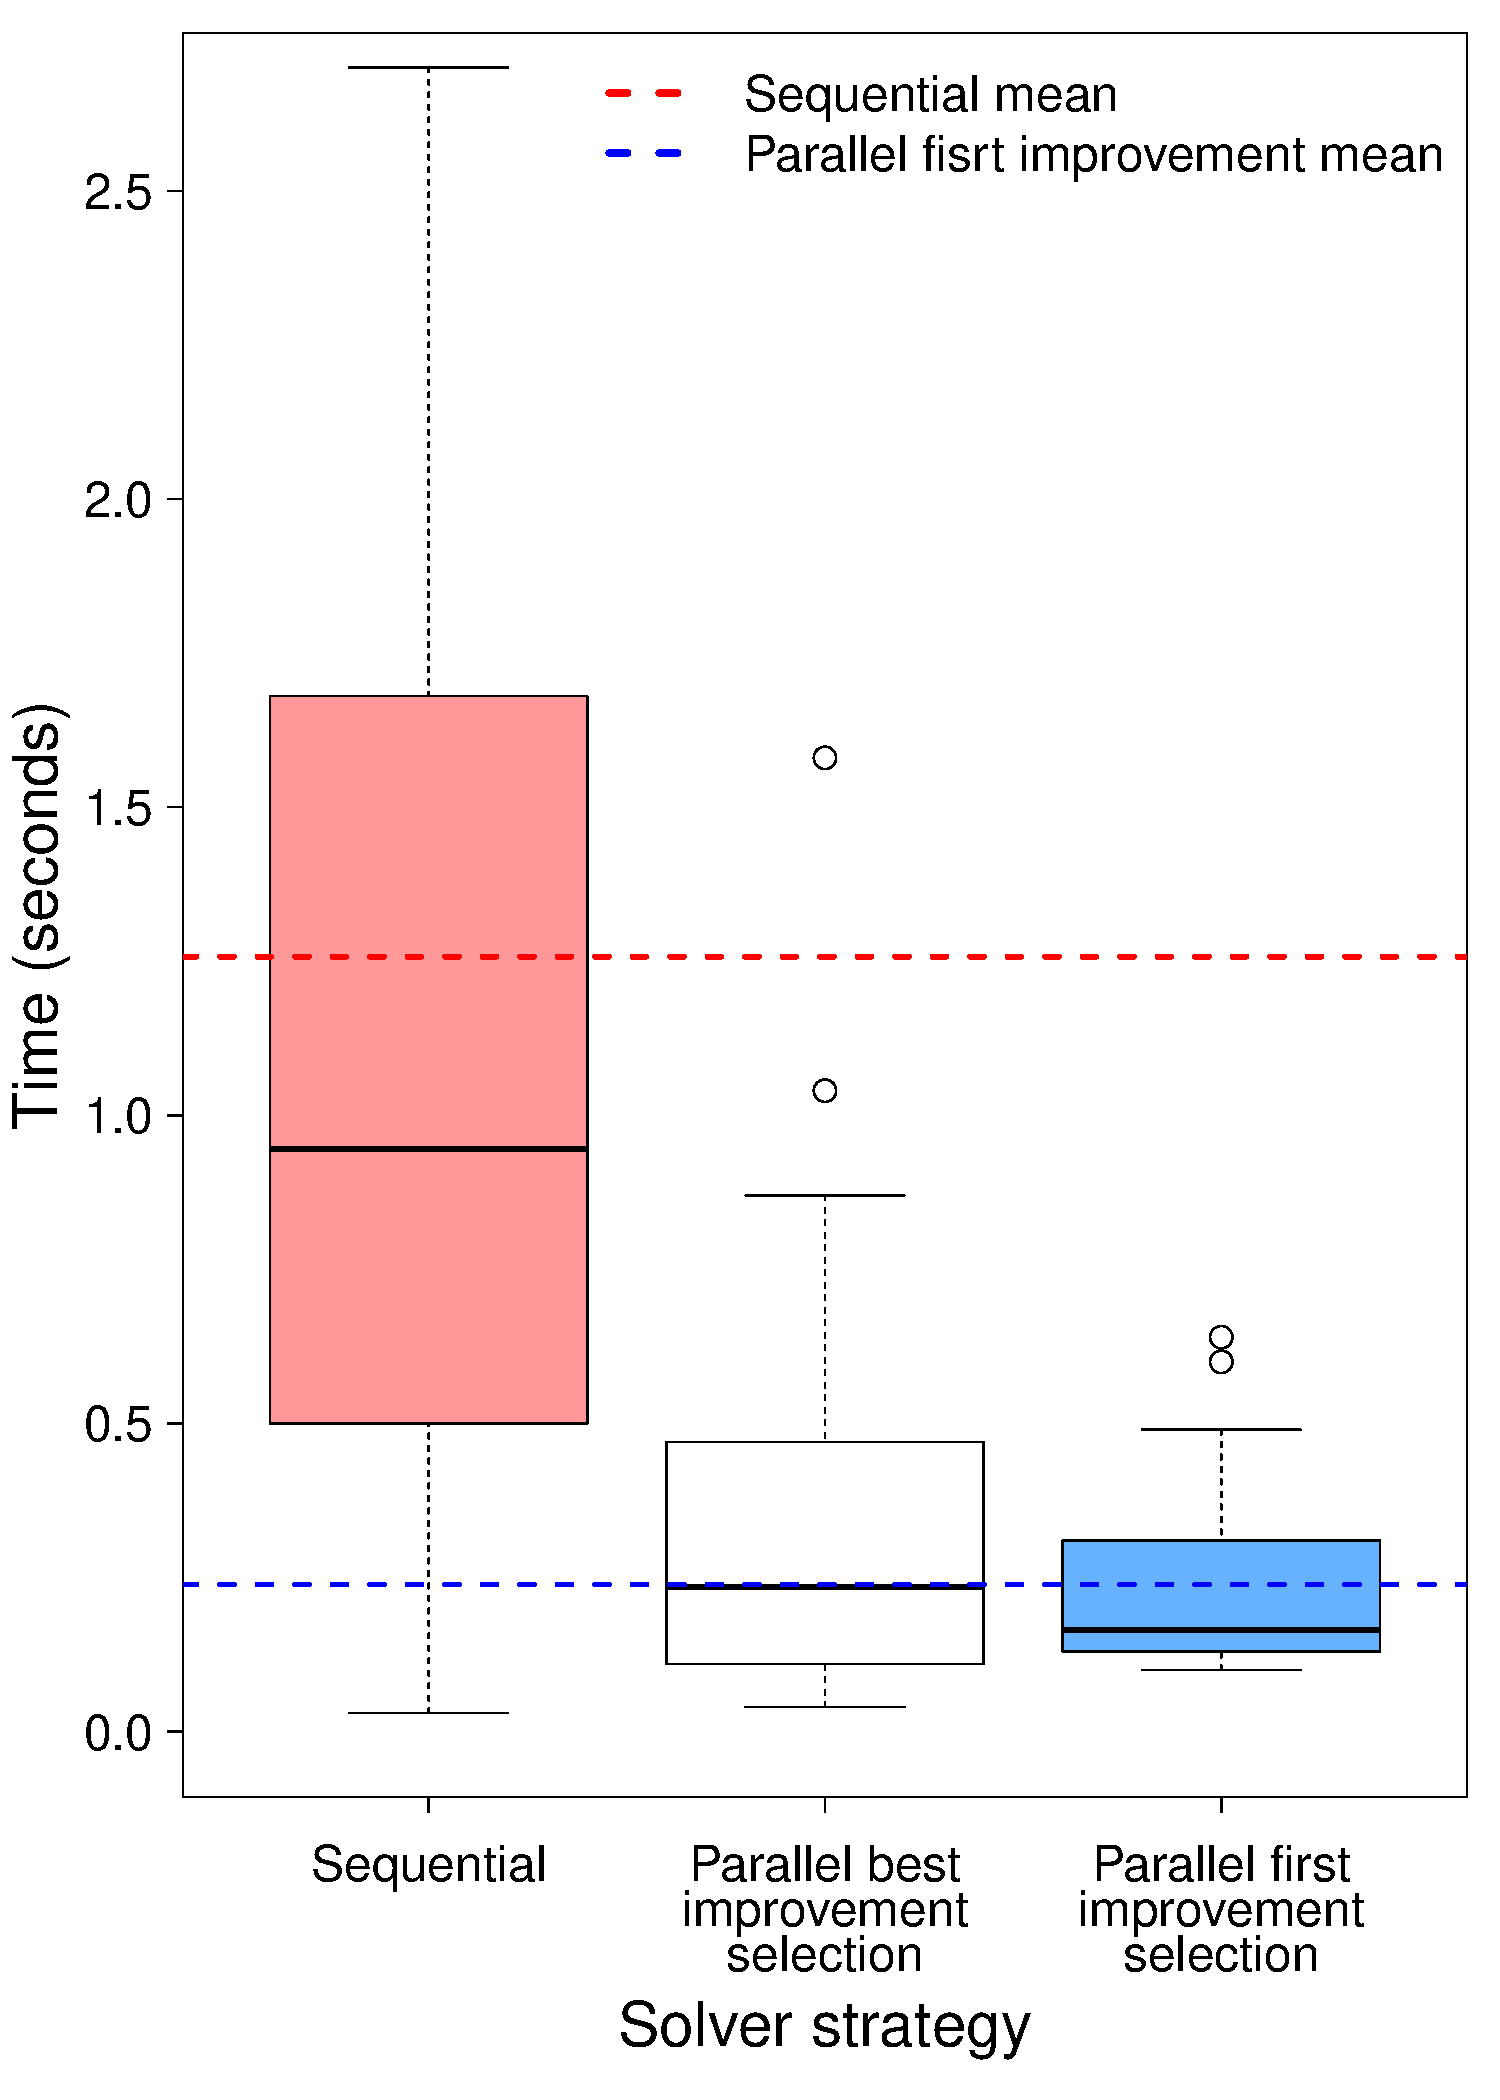
\includegraphics[width=0.4\linewidth]{g5_select_BP.pdf}
%\caption{Comparison between sequential and parallel (best improvement and first improvement selections) runs to solve \SGP{} 5-3-7 using \posl}\label{subfig:boxplot_sel5}
%\end{figure}

\begin{minipage}[c]{0.50\textwidth}
Figures~\ref{subfig:boxplot_sel5}, \ref{subfig:boxplot_sel8} and \ref{subfig:boxplot_sel9} show the huge difference between the spread in results of sequential and parallel runs. Although both parallel strategies (best and first improvement) are equally stable, the one using the selection \om{} of first improvement shows better results: all of their runs are under the mean value of sequential runs (except a suspected outlier).
\end{minipage}\hspace{0.05\textwidth}
\begin{minipage}[c]{0.40\textwidth}
\centering
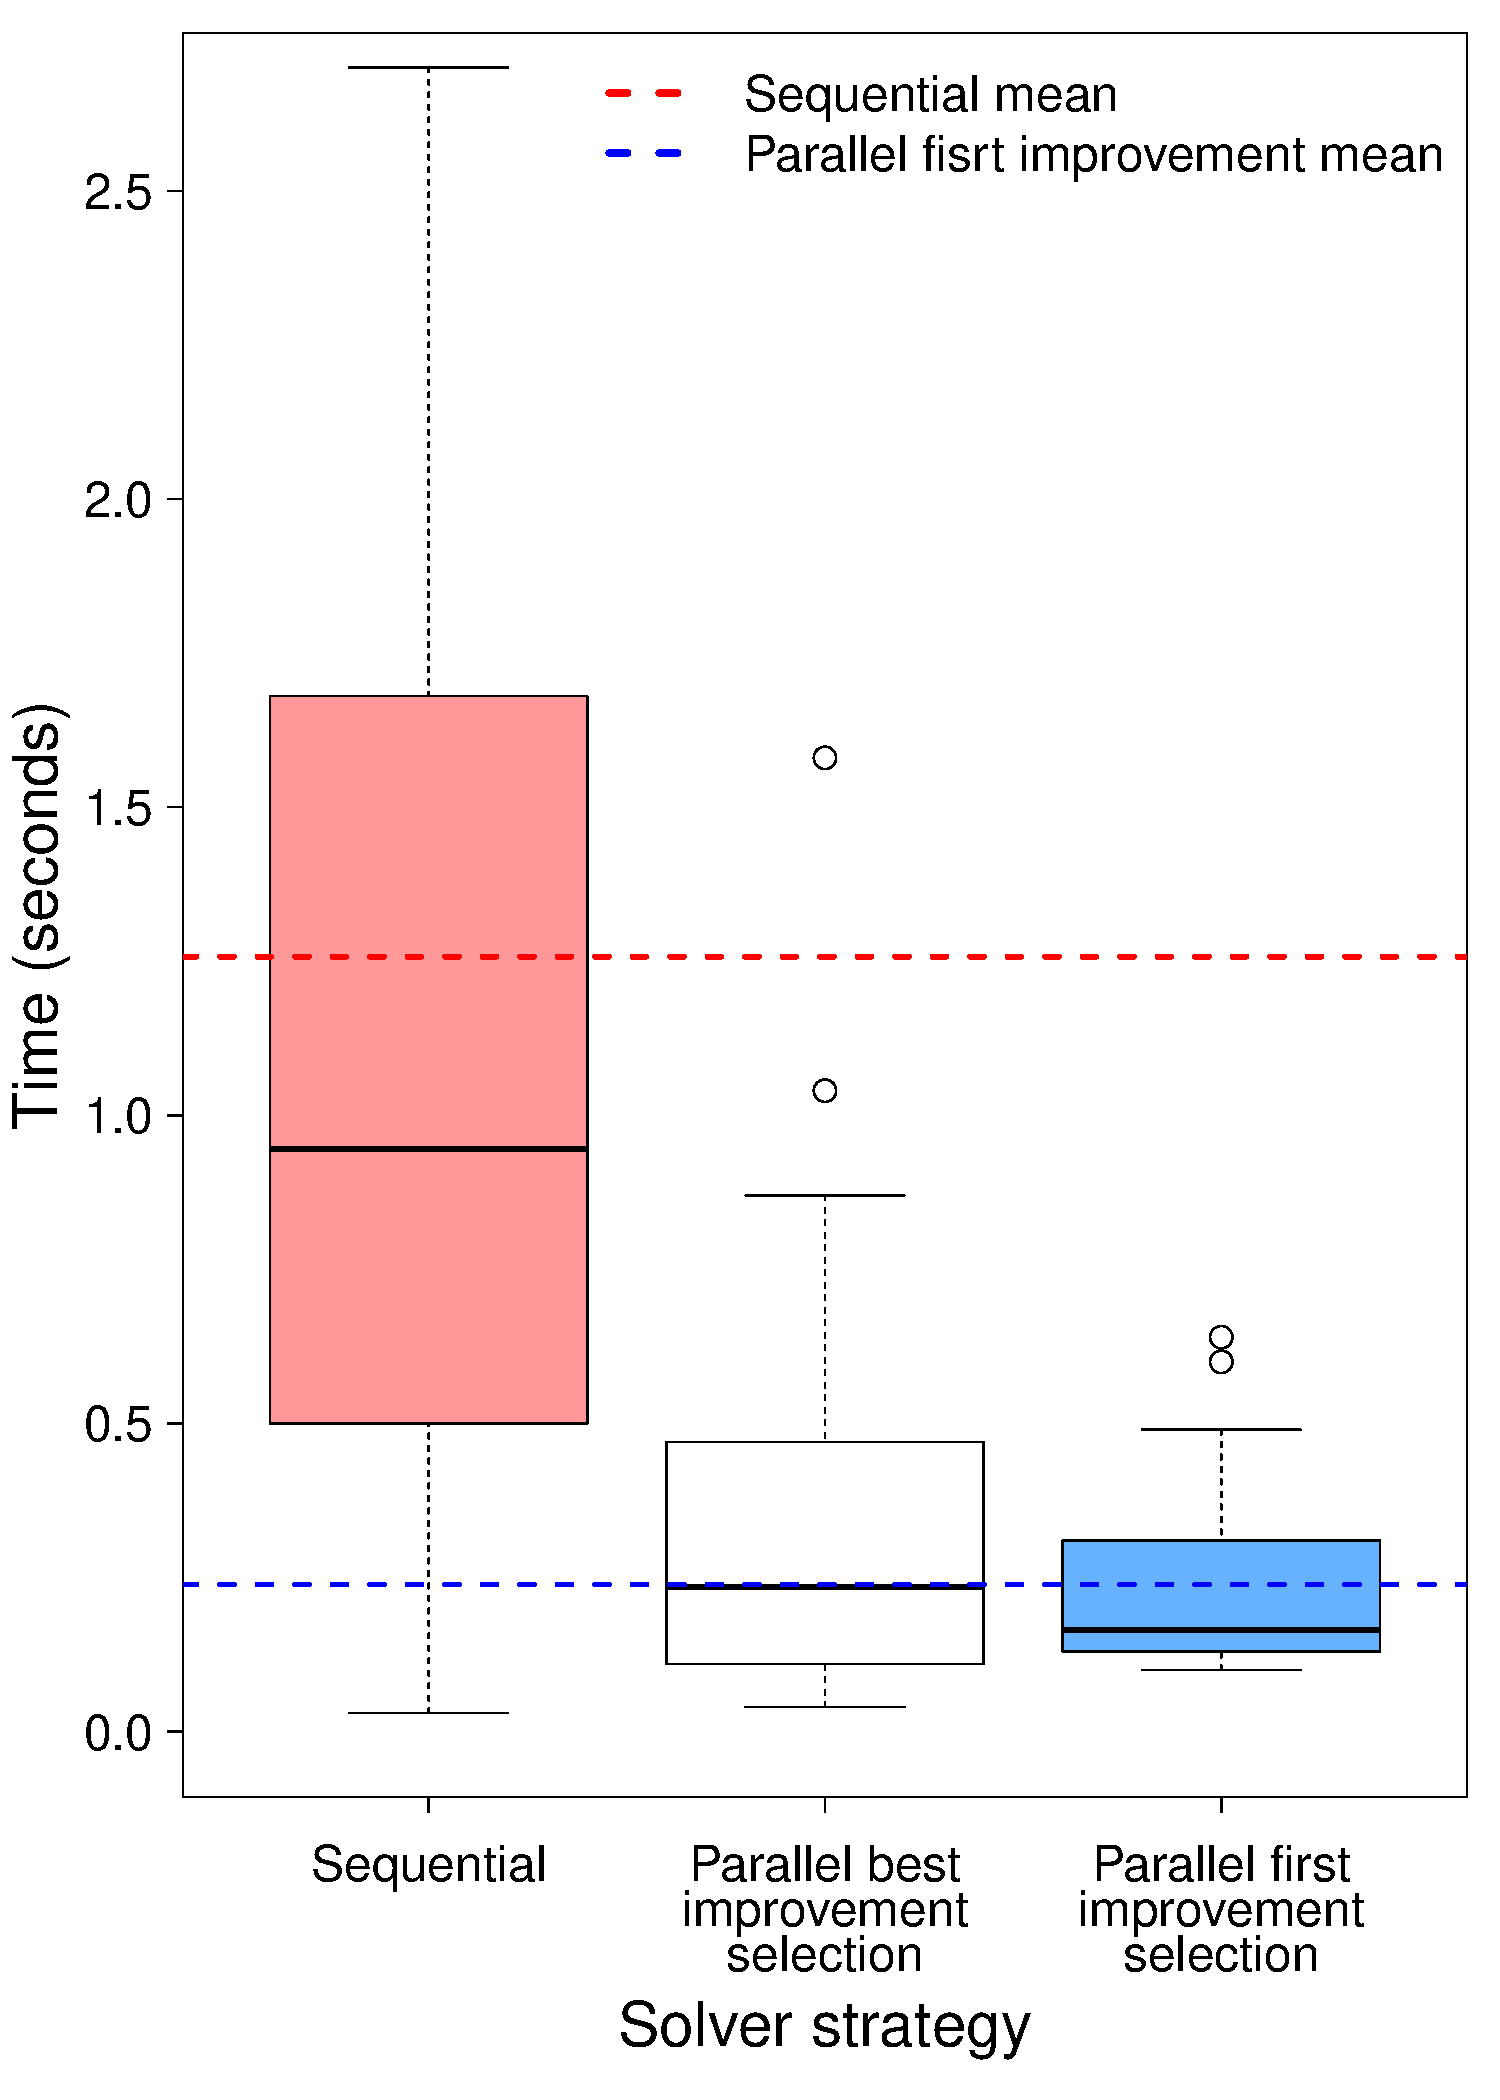
\includegraphics[width=0.9\linewidth]{g5_select_BP.pdf}
\captionof{figure}{Comparison between sequential and parallel (best improvement and first improvement selections) runs to solve \SGP{} 5-3-7 using \posl}\label{subfig:boxplot_sel5}
\end{minipage}

\begin{minipage}[c]{0.45\textwidth}
\centering
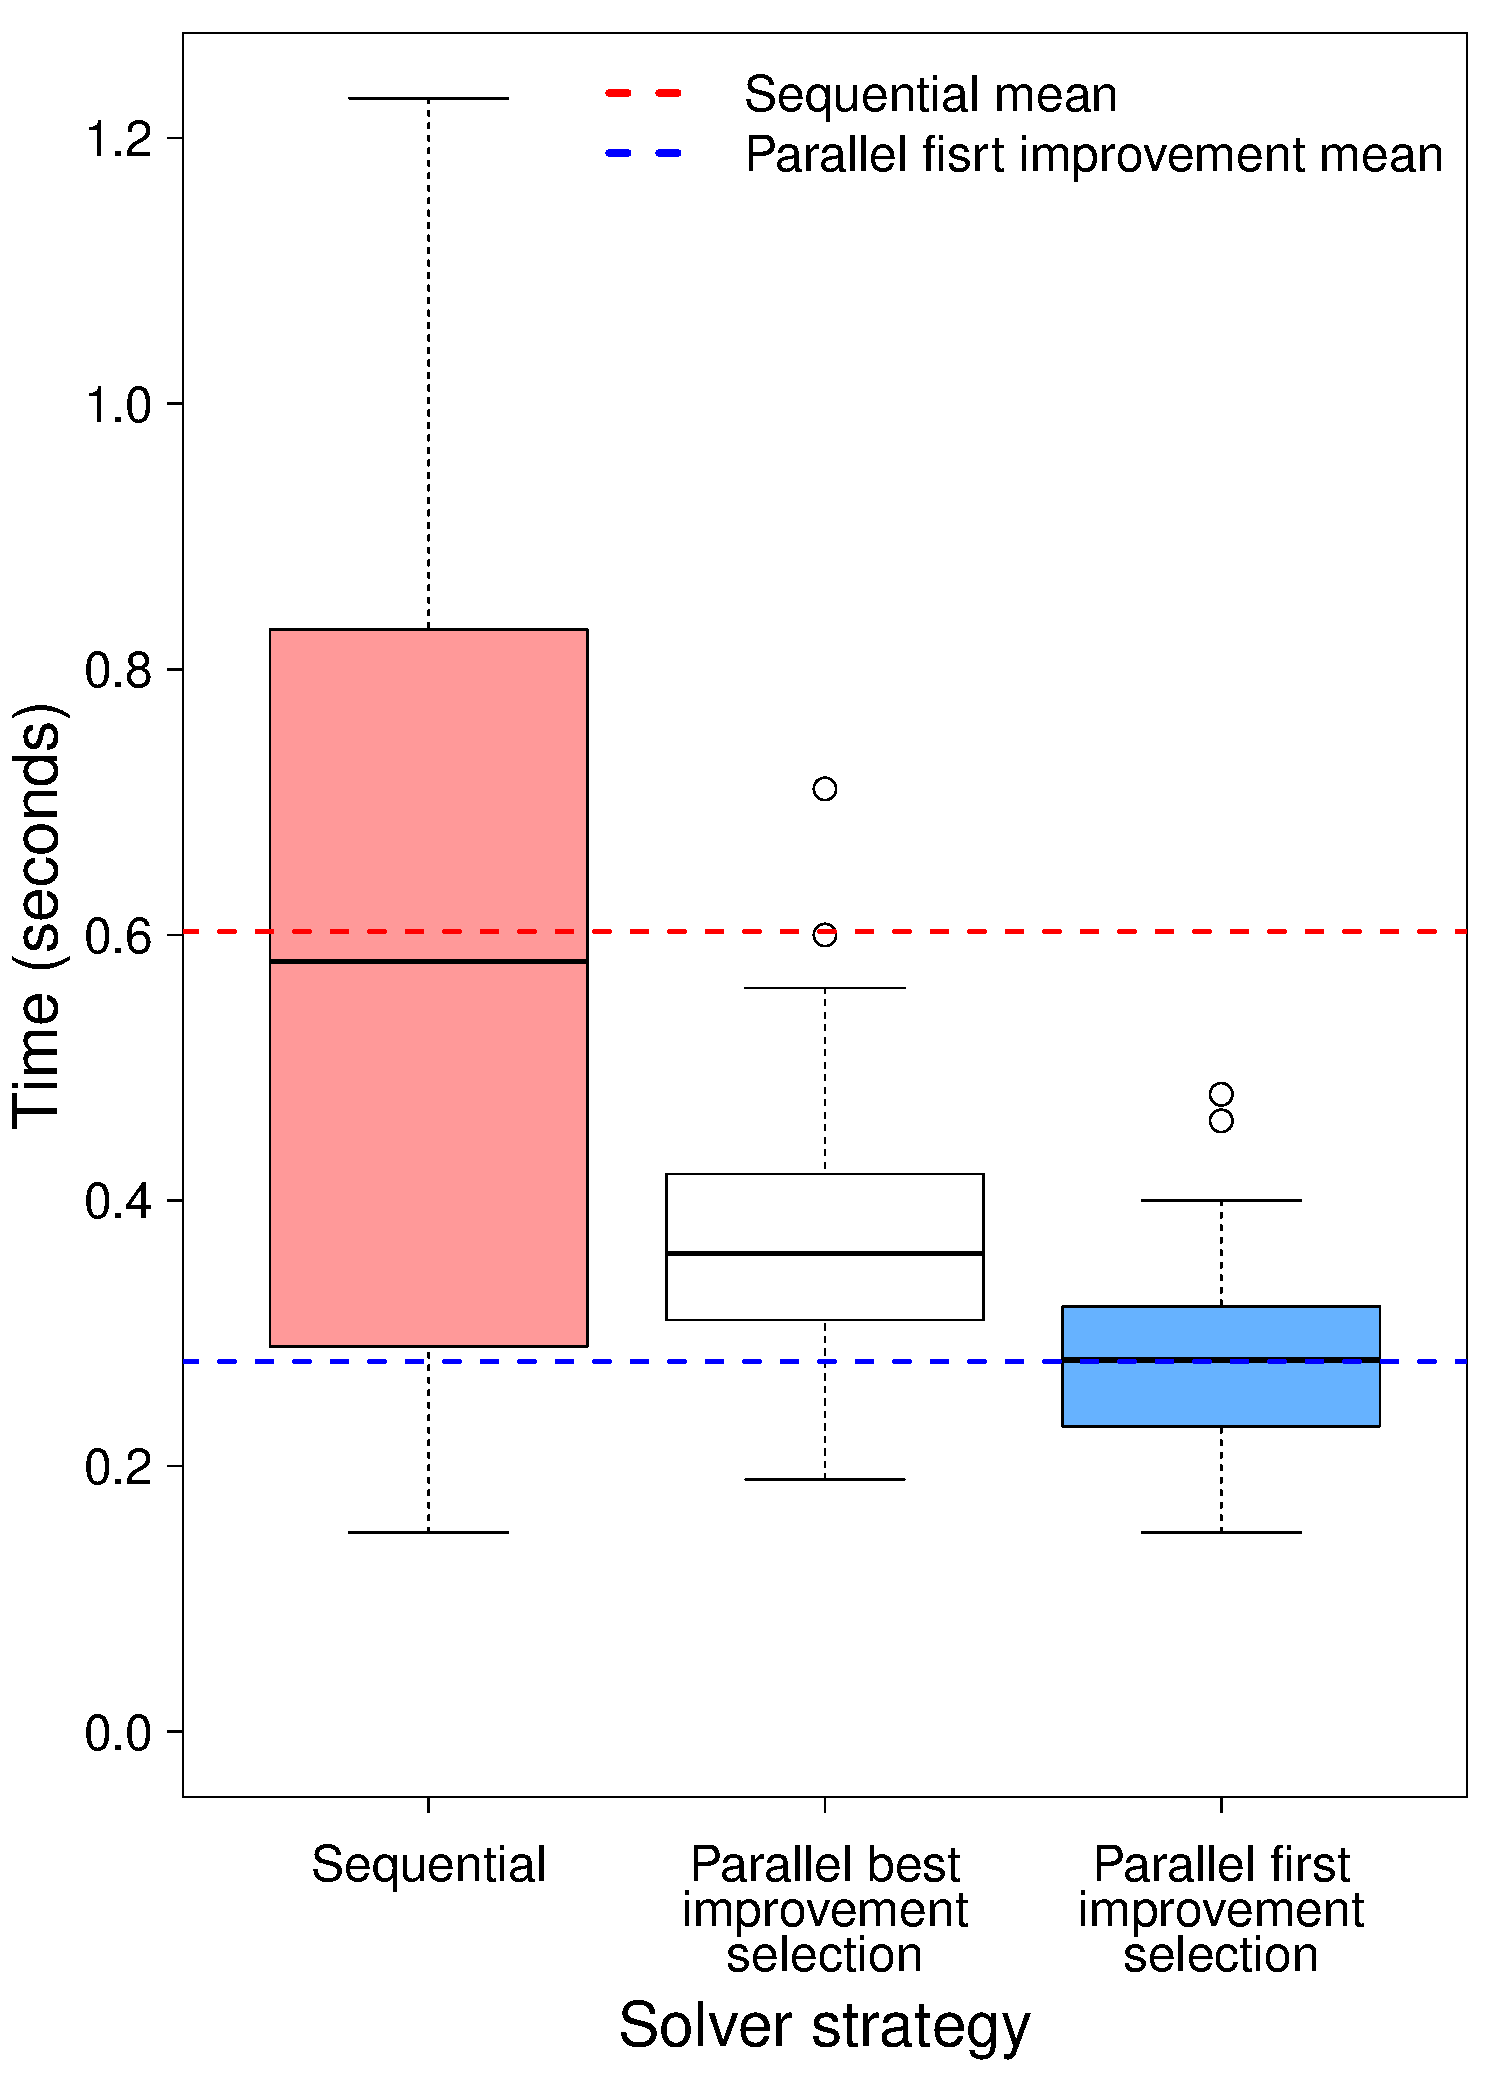
\includegraphics[width=\linewidth]{g8_select_BP.pdf}
\captionof{figure}{Comparison between sequential and parallel (best improvement and first improvement selections) runs to solve \SGP{} 8-4-7 using \posl}\label{subfig:boxplot_sel8}
\end{minipage}\hspace{0.05\textwidth}
\begin{minipage}[c]{0.45\textwidth}
\centering
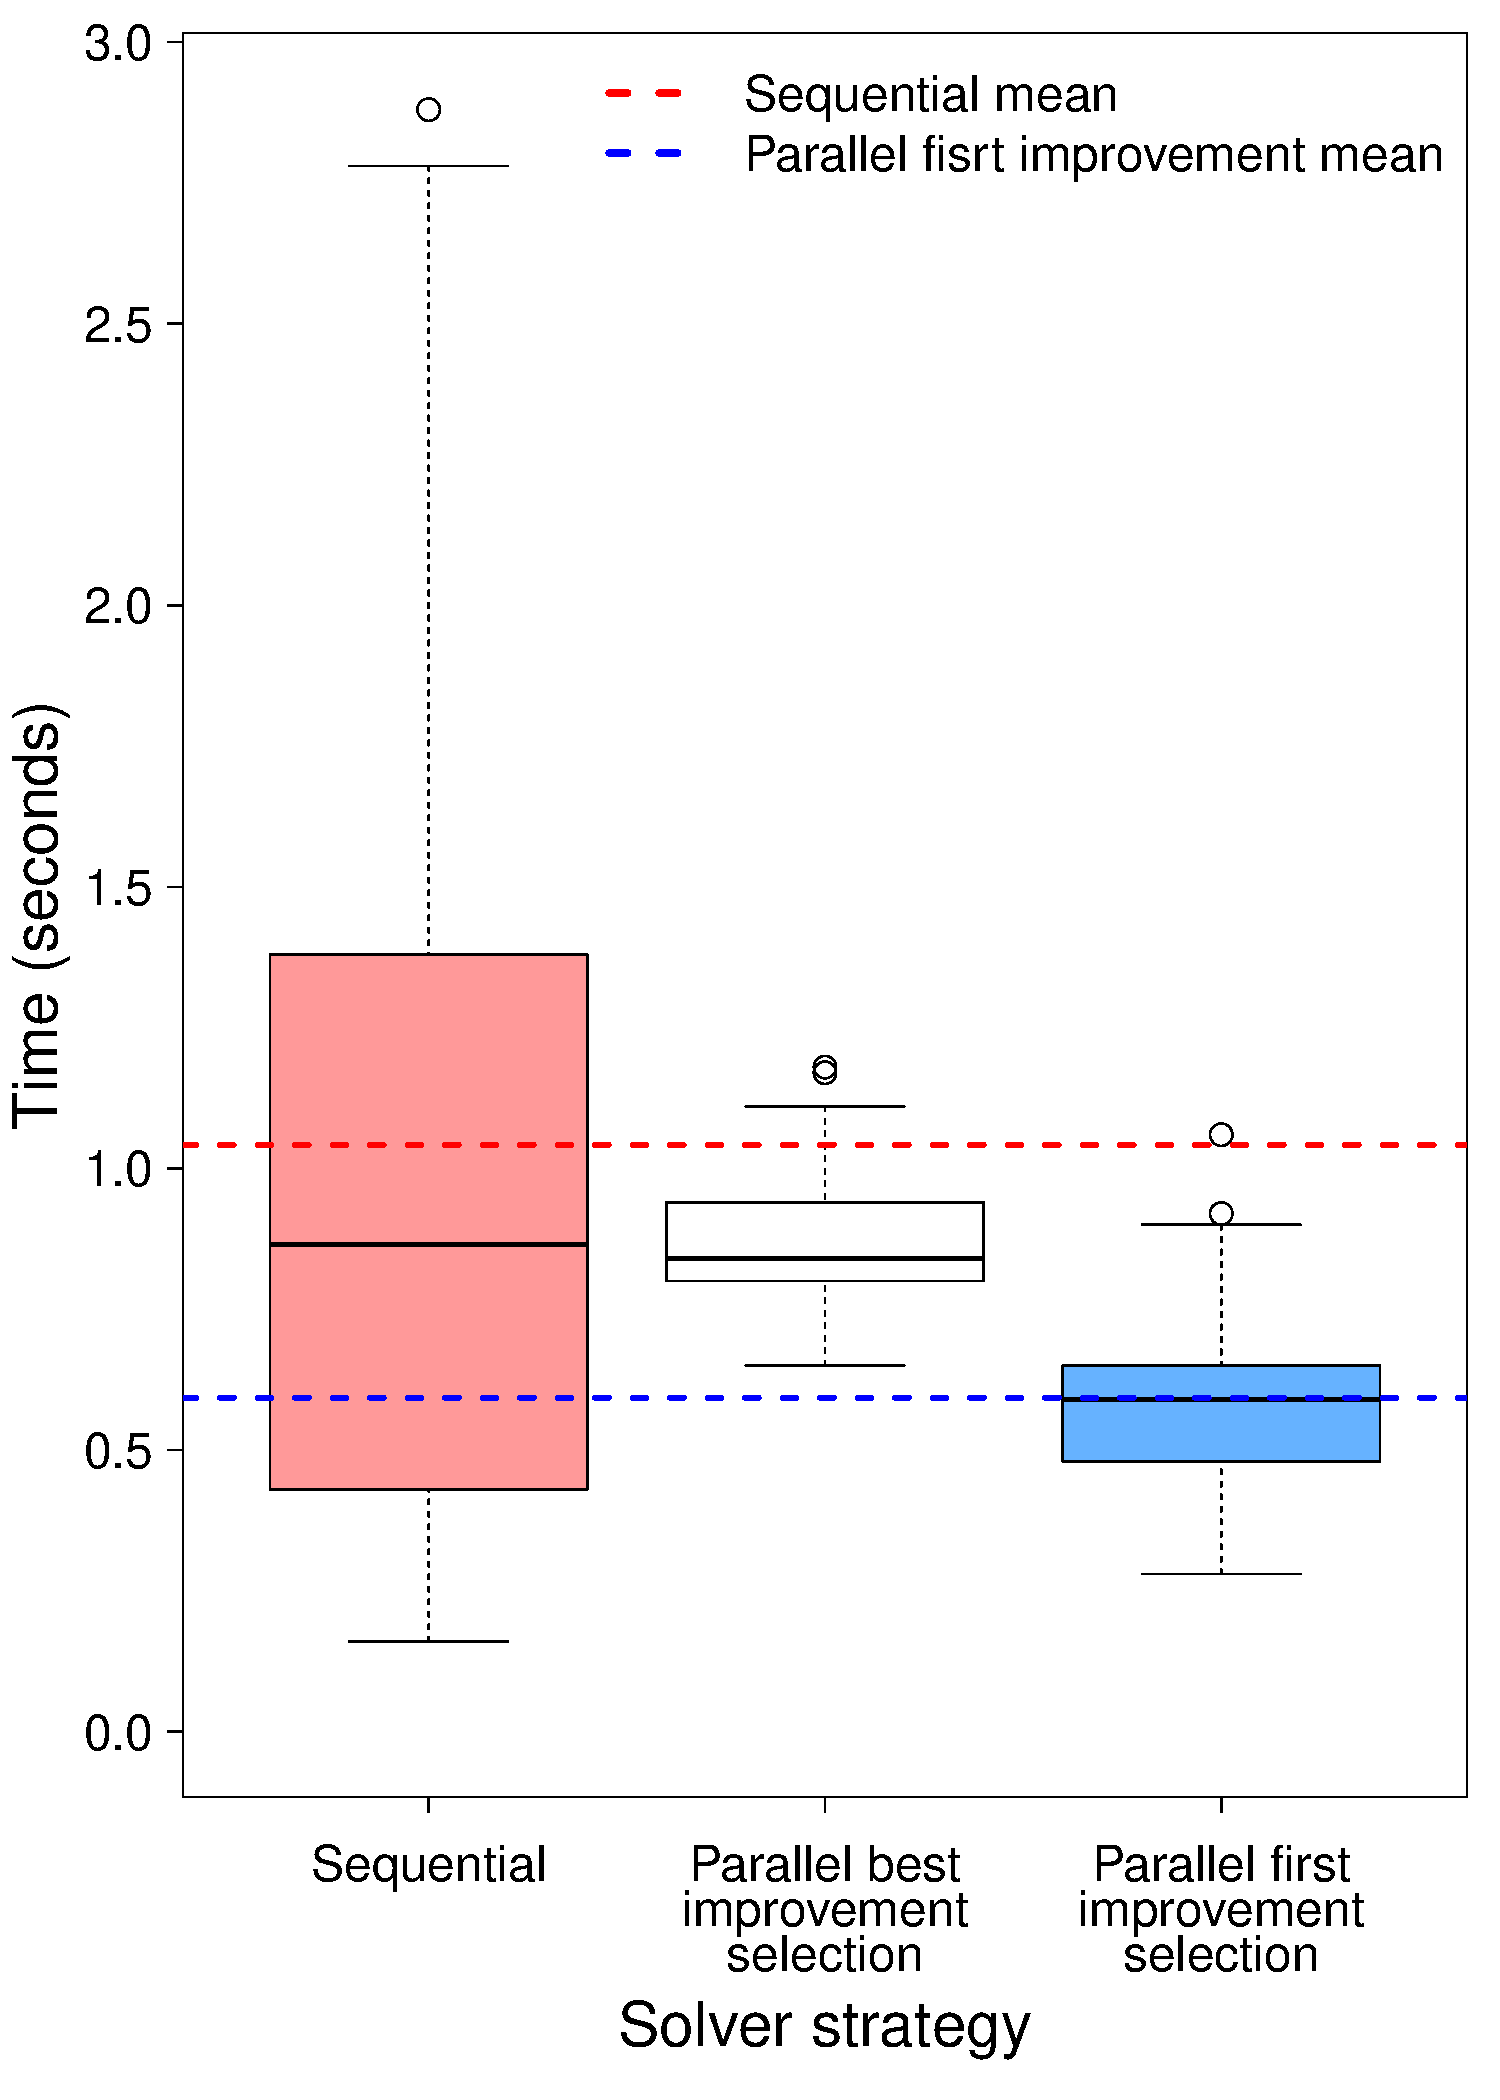
\includegraphics[width=\linewidth]{g9_select_BP.pdf}
\captionof{figure}{Comparison between sequential and parallel (best improvement and first improvement selections) runs to solve \SGP{} 9-4-8 using \posl}\label{subfig:boxplot_sel9}
\end{minipage}

\section{Comparison between \commstrs}

In Figures~\ref{boxplot:5comm}, \ref{boxplot:8comm} and \ref{boxplot:9comm}, labels of the x-axis correspond to the following strategies:

\poslcaptiondesciption{
\begin{tabular}[t]{rl}
\textbf{NC}: & \begin{tabular}[t]{l} Non communication strategy \end{tabular} \\
%\textbf{NC}: & Non communication strategy\\
\textbf{100SC1-1}: & \begin{tabular}[t]{l} 100\% of communicating solvers performing simple communication \oneTone \end{tabular} \\
\textbf{50SC1-1}: & \begin{tabular}[t]{l} 50\% of communicating solvers performing simple communication \oneTone \end{tabular} \\
\textbf{25SC1-1}: & \begin{tabular}[t]{l} 25\% of communicating solvers performing simple communication \oneTone \end{tabular} \\
\textbf{100SC1-n}: & \begin{tabular}[t]{l} 100\% of communicating solvers performing simple communication \oneTn \end{tabular} \\
\textbf{50SC1-n}: & \begin{tabular}[t]{l} 50\% of communicating solvers performing simple communication \oneTn \end{tabular} \\
\textbf{25SC1-n}: & \begin{tabular}[t]{l} 25\% of communicating solvers performing simple communication \oneTn \end{tabular}\\
\textbf{CC1-n}: & \begin{tabular}[t]{l} One set of solvers performing dynamic exchange communication \oneTn \end{tabular} \\
\textbf{CC1-n/2}: & \begin{tabular}[t]{l} Two sets of solvers performing dynamic exchange communication \oneTn \end{tabular} \\
\textbf{CC1-n/4}: & \begin{tabular}[t]{l} Four sets of solvers performing dynamic exchange communication \oneTn \end{tabular} \\
\textbf{100CC1-1}: & \begin{tabular}[t]{l} 100\% of communicating solvers performing dynamic exchange communication \\ \oneTone \end{tabular}\\
\textbf{50CC1-1}: & \begin{tabular}[t]{l} 50\% of communicating solvers performing dynamic exchange communication \\ \oneTone \end{tabular} \\
\textbf{25CC1-1}: & \begin{tabular}[t]{l} 25\% of communicating solvers performing dynamic exchange communication \\ \oneTone \end{tabular}\\
\end{tabular}
}

%\begin{figure}[h]
\begin{minipage}[c]{\textwidth}
\centering
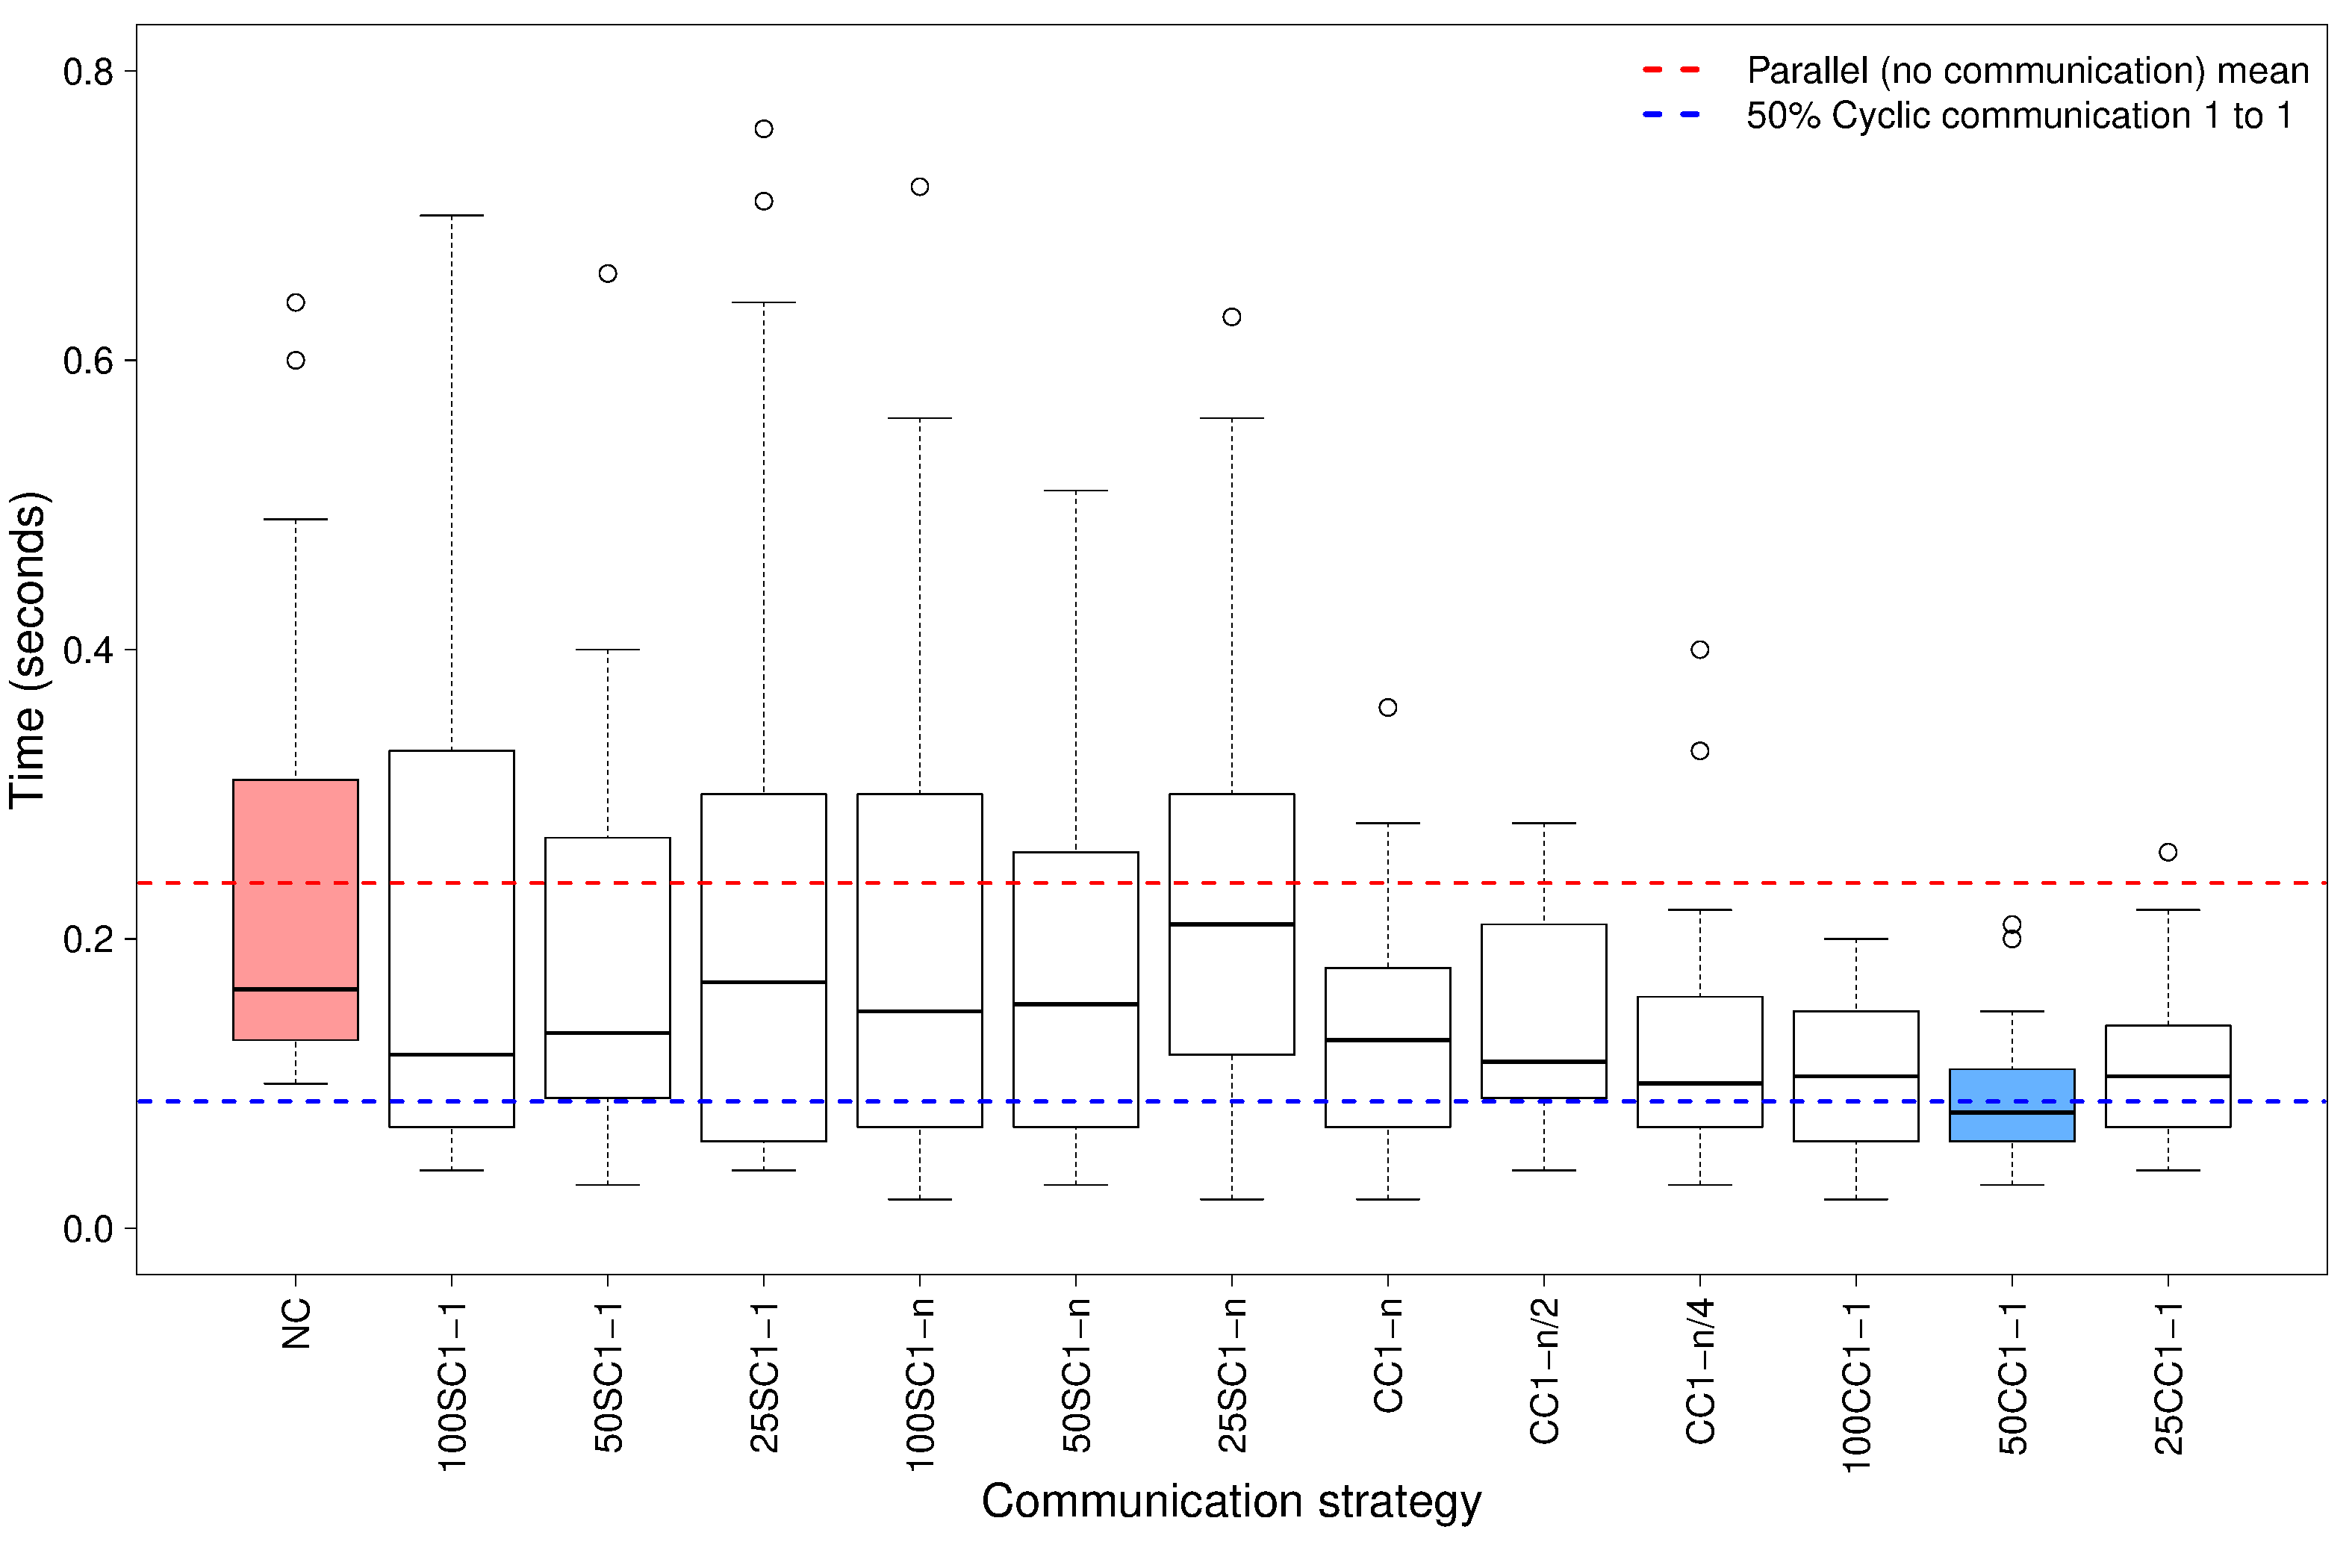
\includegraphics[width=0.8\textwidth]{g5_comm_BP.pdf}
\captionof{figure}{Different communication strategies to solve \SGP{} 5-3-7 using \posl}\label{boxplot:5comm}
\end{minipage}
%\end{figure}

Figures~\ref{boxplot:5comm}, \ref{boxplot:8comm} and~\ref{boxplot:9comm} show results summaries of different \commstrs{}. They are presented together with the box-plot graph of parallel results without communication (\texttt{NC}). In all cases we can observe that strategies \texttt{100\%CC1-1} and \texttt{50\%CC1-1}  show excellent results in comparison to the one without communication. This figure shows also that simple \commstrs{} do not contribute enough to the improvement of the search time.


\begin{minipage}[c]{\textwidth}
%\begin{figure}[h]
\centering
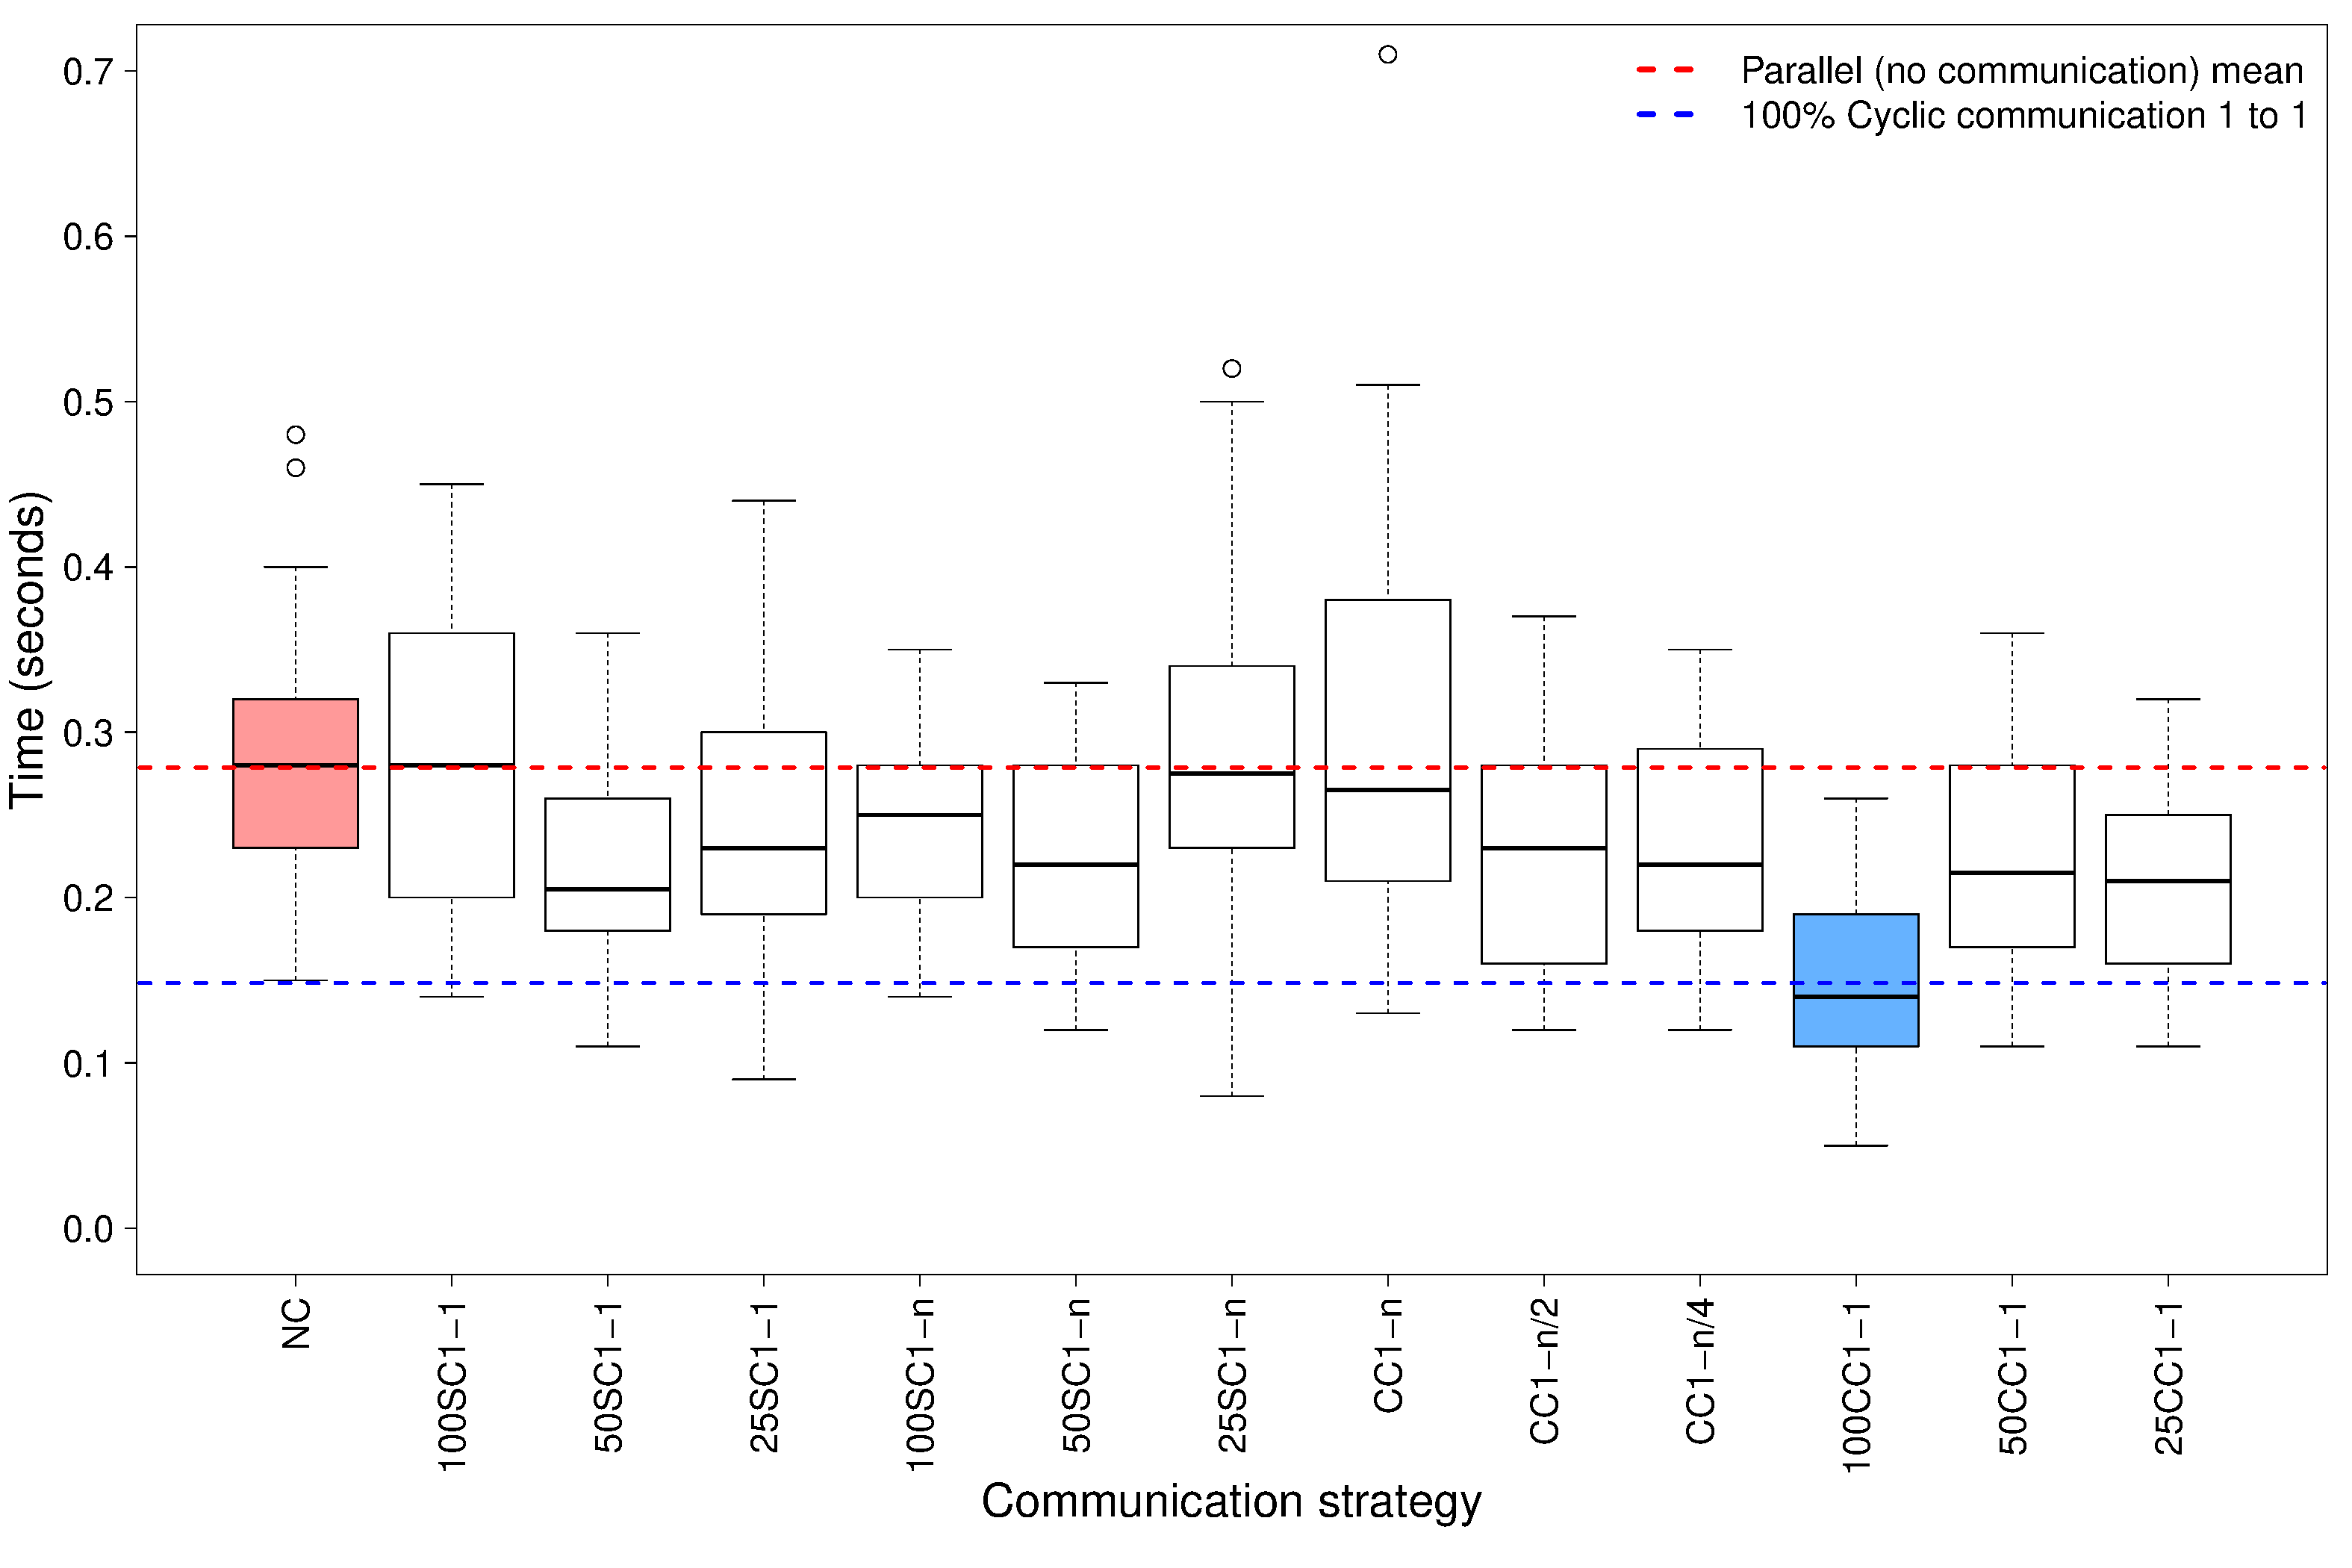
\includegraphics[width=0.75\textwidth]{g8_comm_BP.pdf}
\captionof{figure}{Different communication strategies to solve \SGP{} 8-4-7 using \posl}\label{boxplot:8comm}
\end{minipage}
%\end{figure}

\begin{minipage}[c]{\textwidth}
%\begin{figure}[h]
\centering
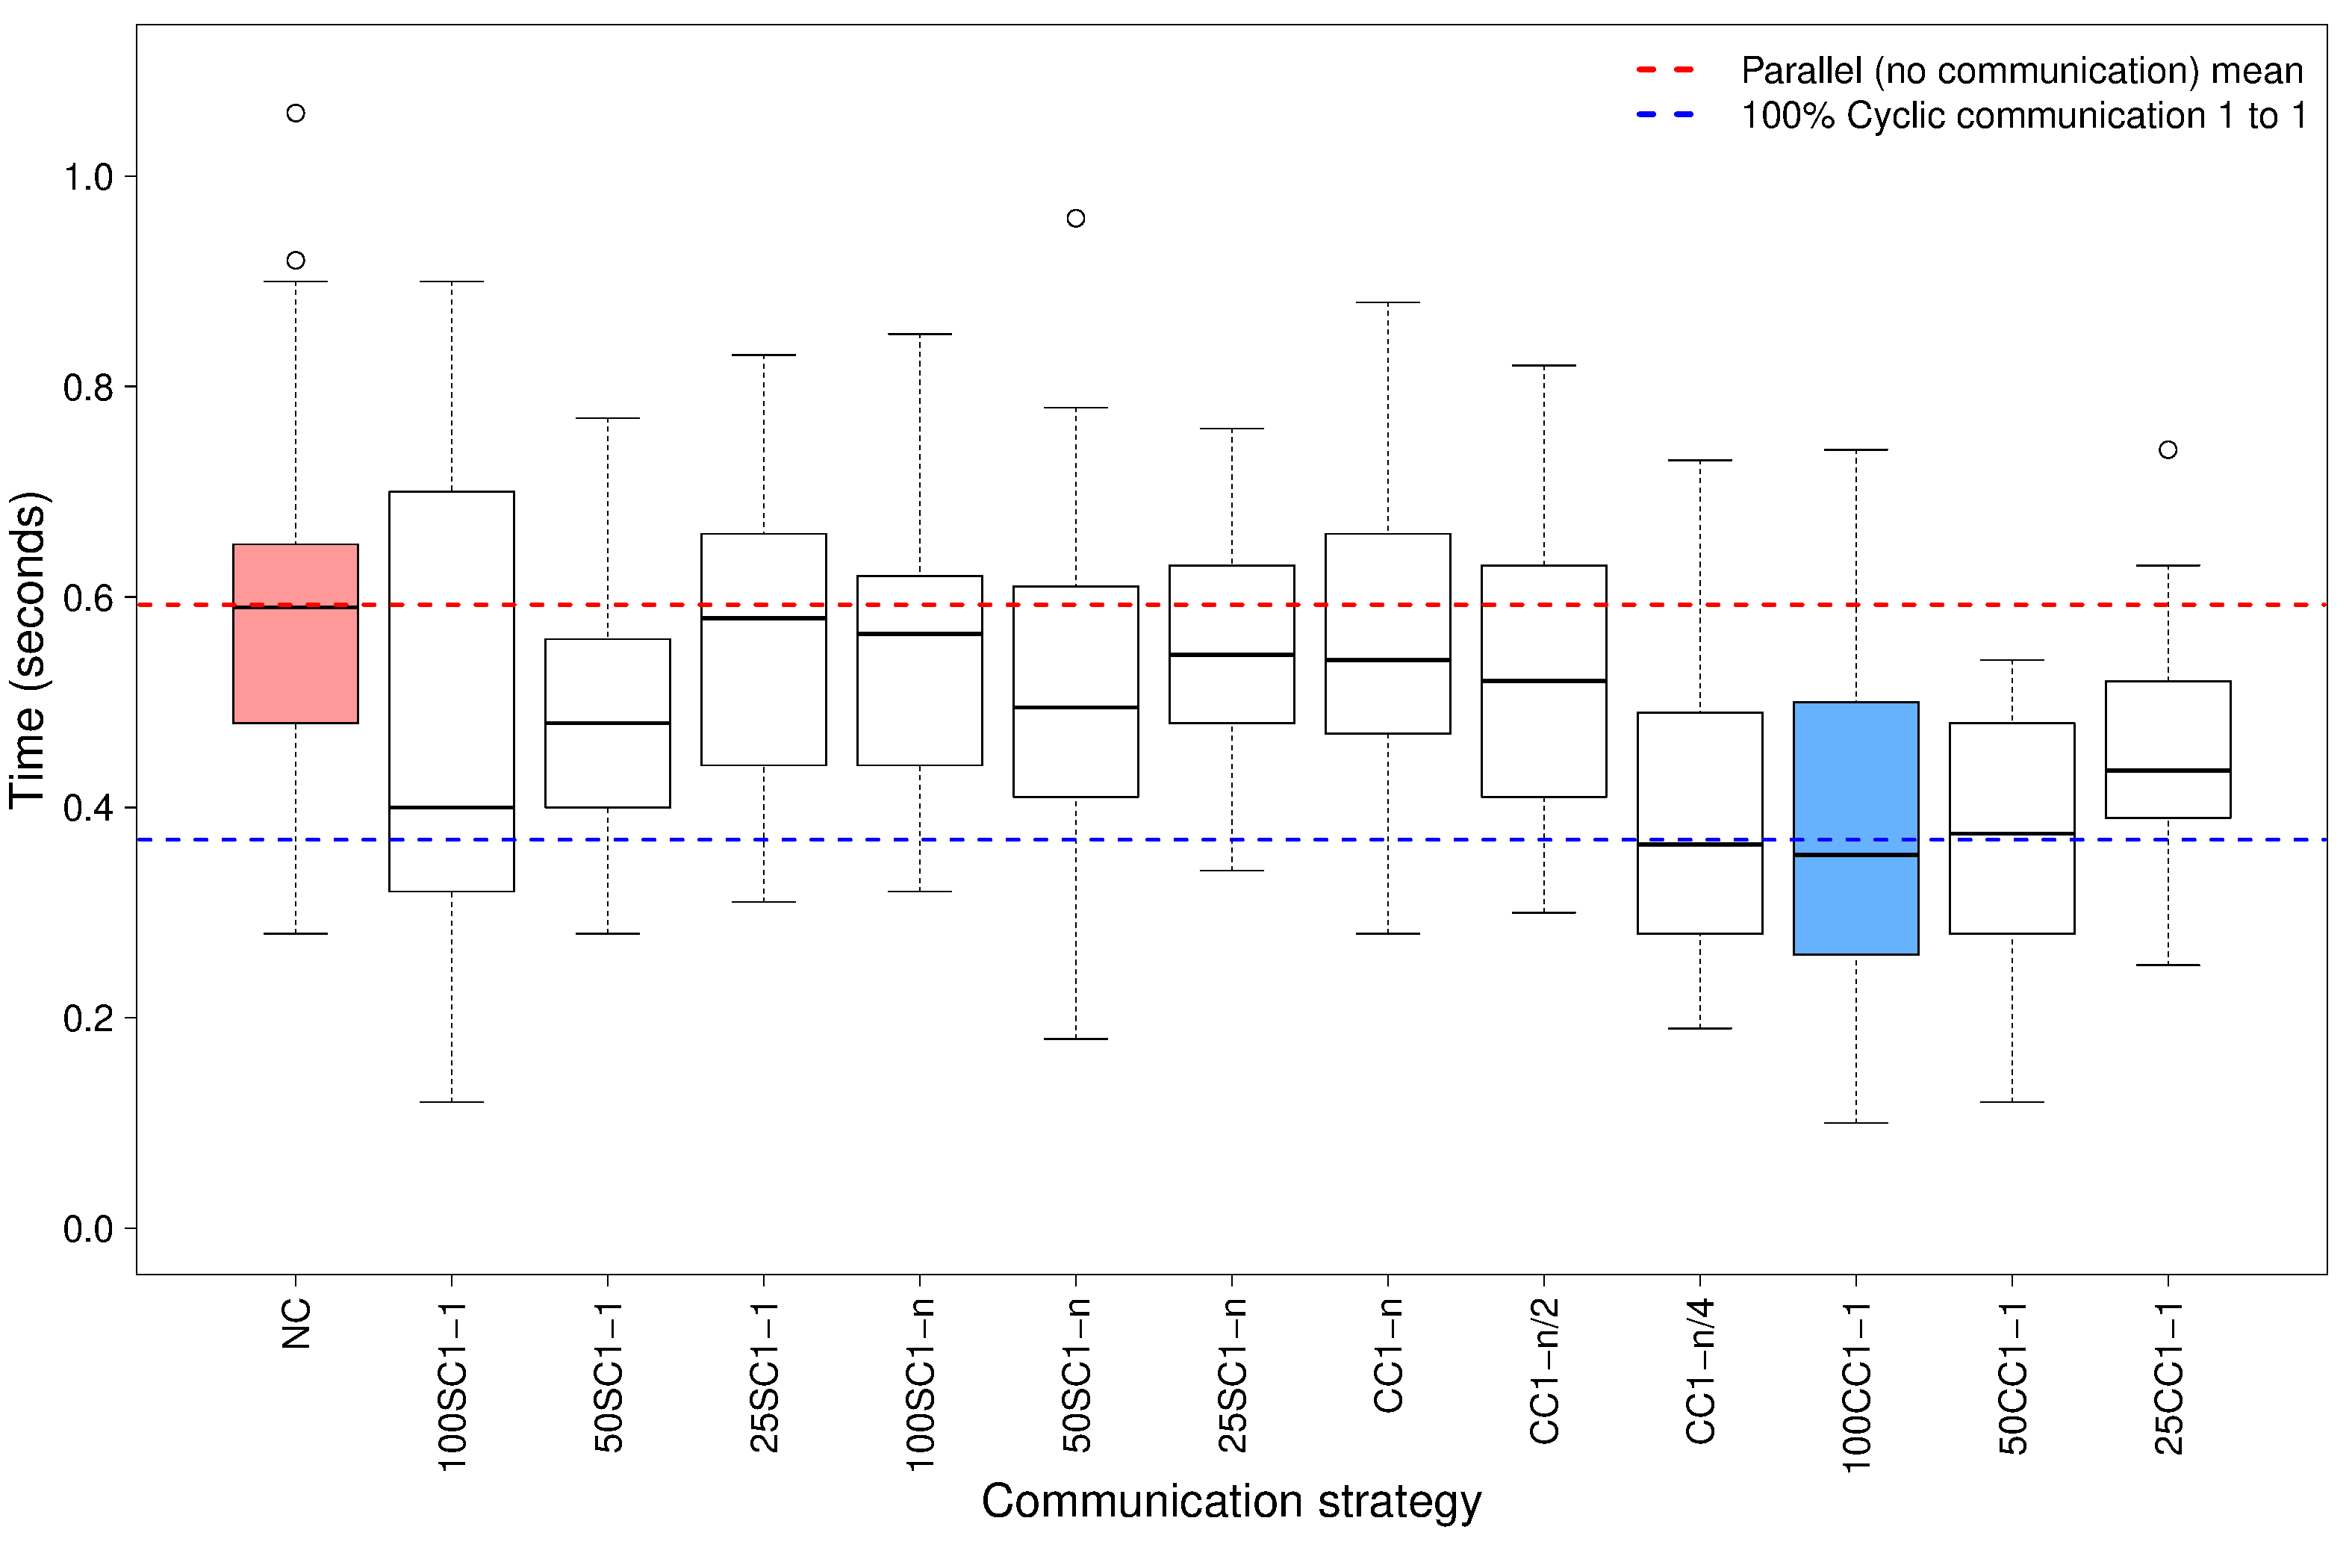
\includegraphics[width=0.75\textwidth]{g9_comm_BP.pdf}
\captionof{figure}{Different communication strategies to solve \SGP{} 9-4-8 using \posl}\label{boxplot:9comm}
%\end{figure}
\end{minipage}

%\begin{figure}[!h]
%\centering
%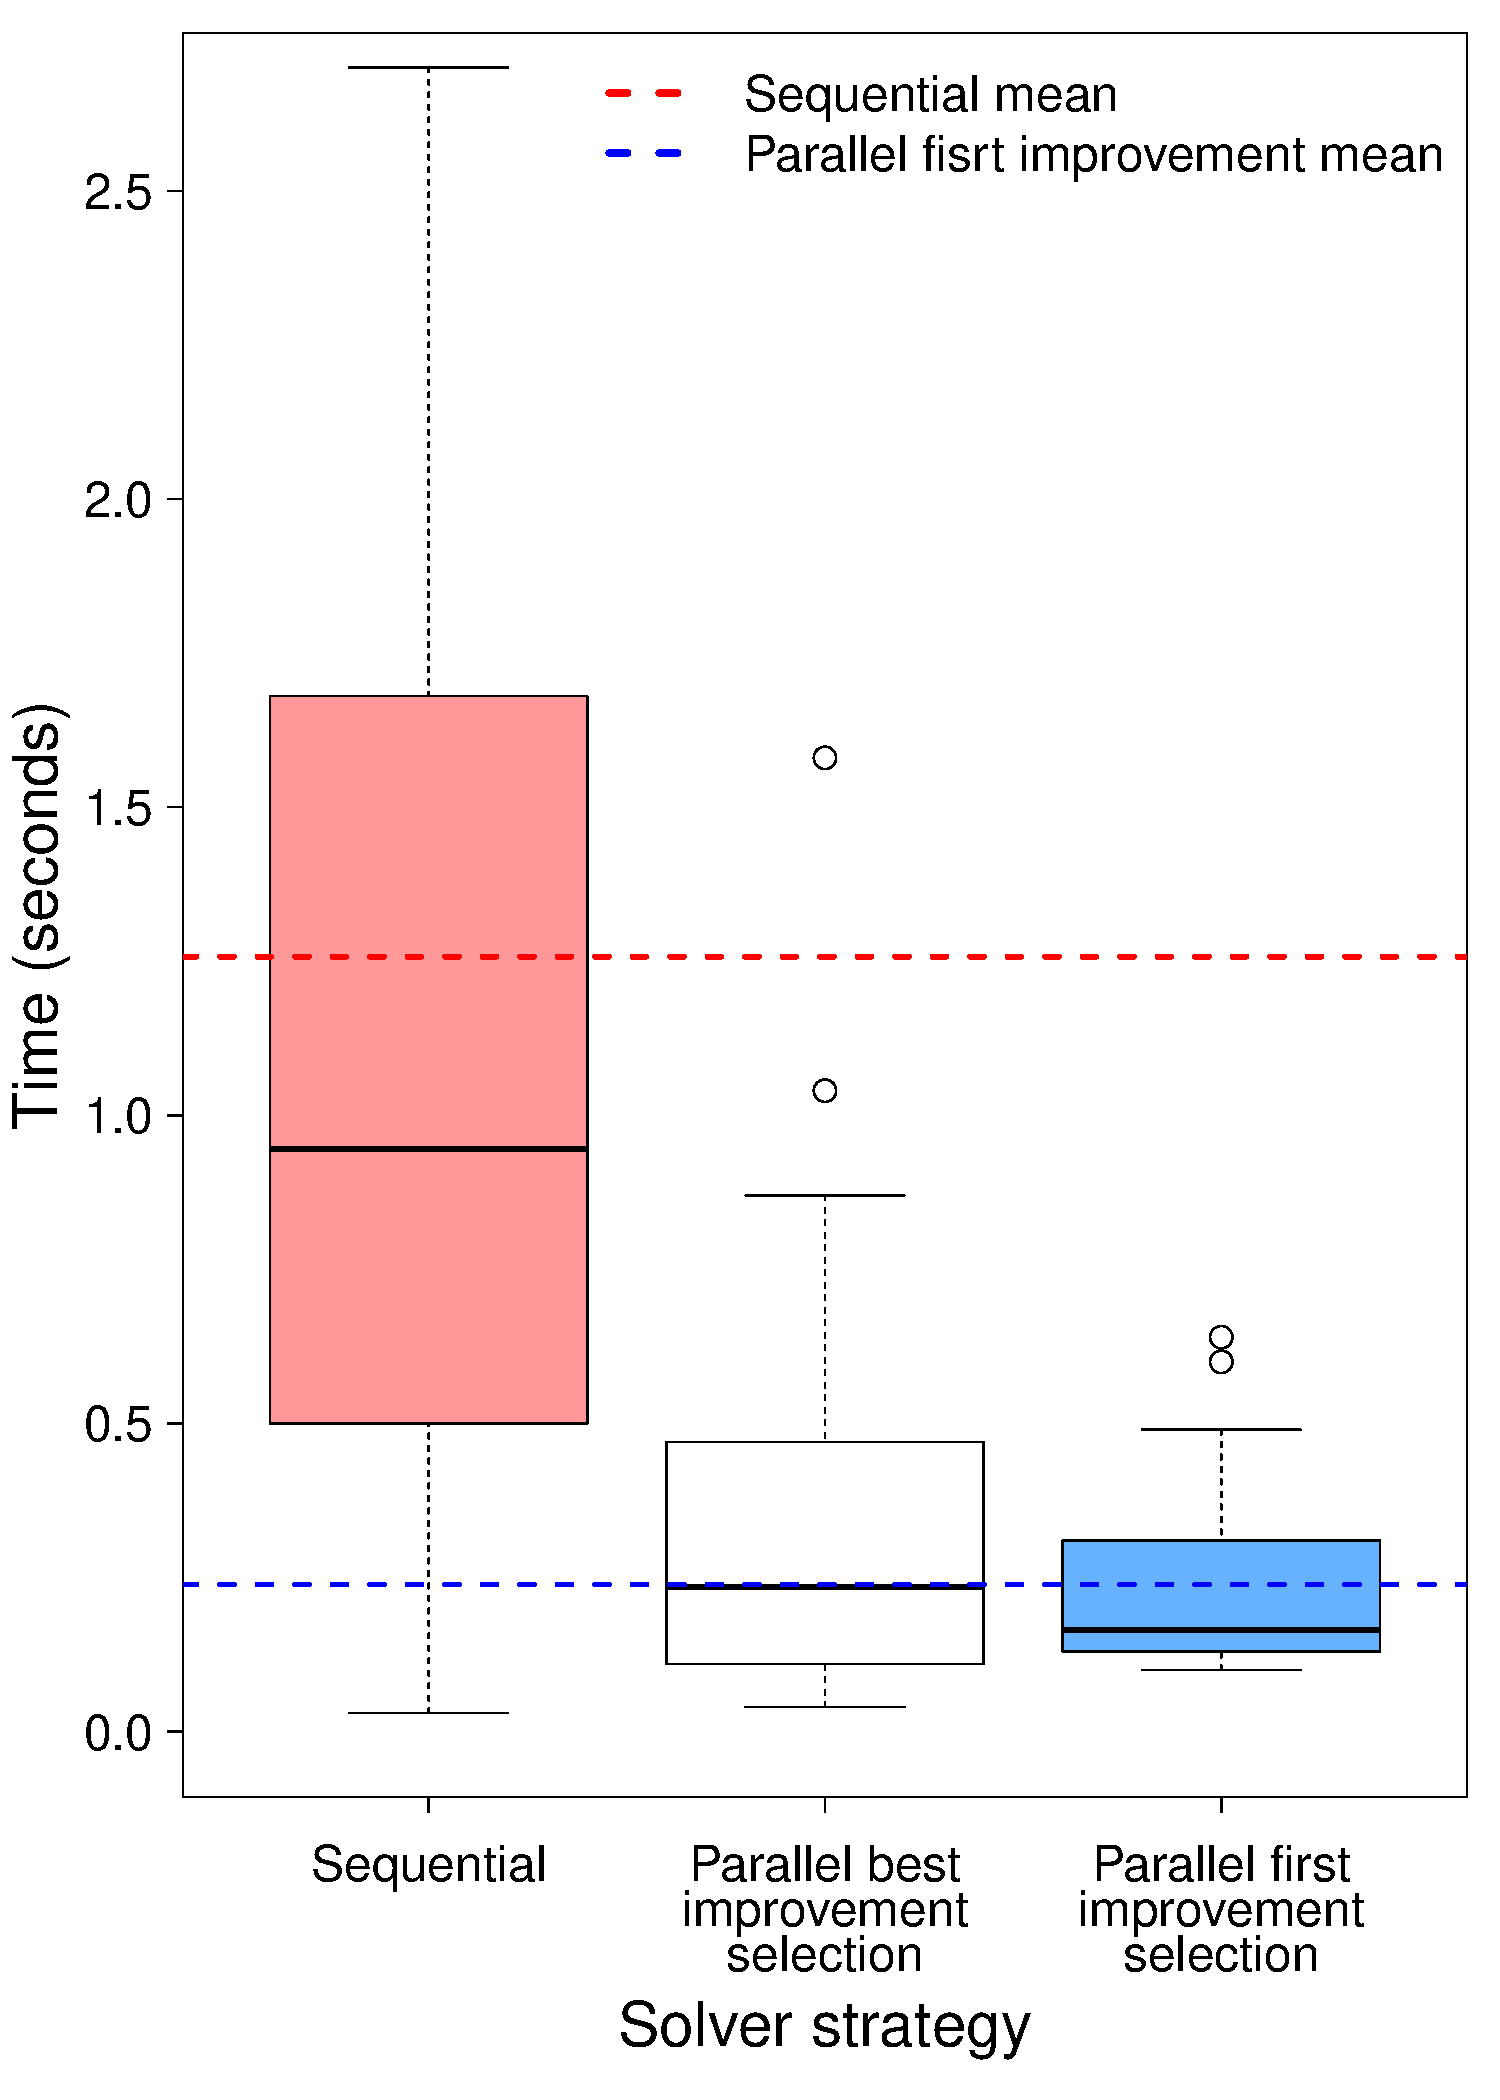
\includegraphics[width=0.4\textwidth]{g5_select_BP.pdf}
%\caption{Comparison between sequential and parallel (best improvement and first improvement selections) runs to solve \SGP{} 5-3-7 using \posl}
%\end{figure}

%\begin{figure}[!h]
%\centering
%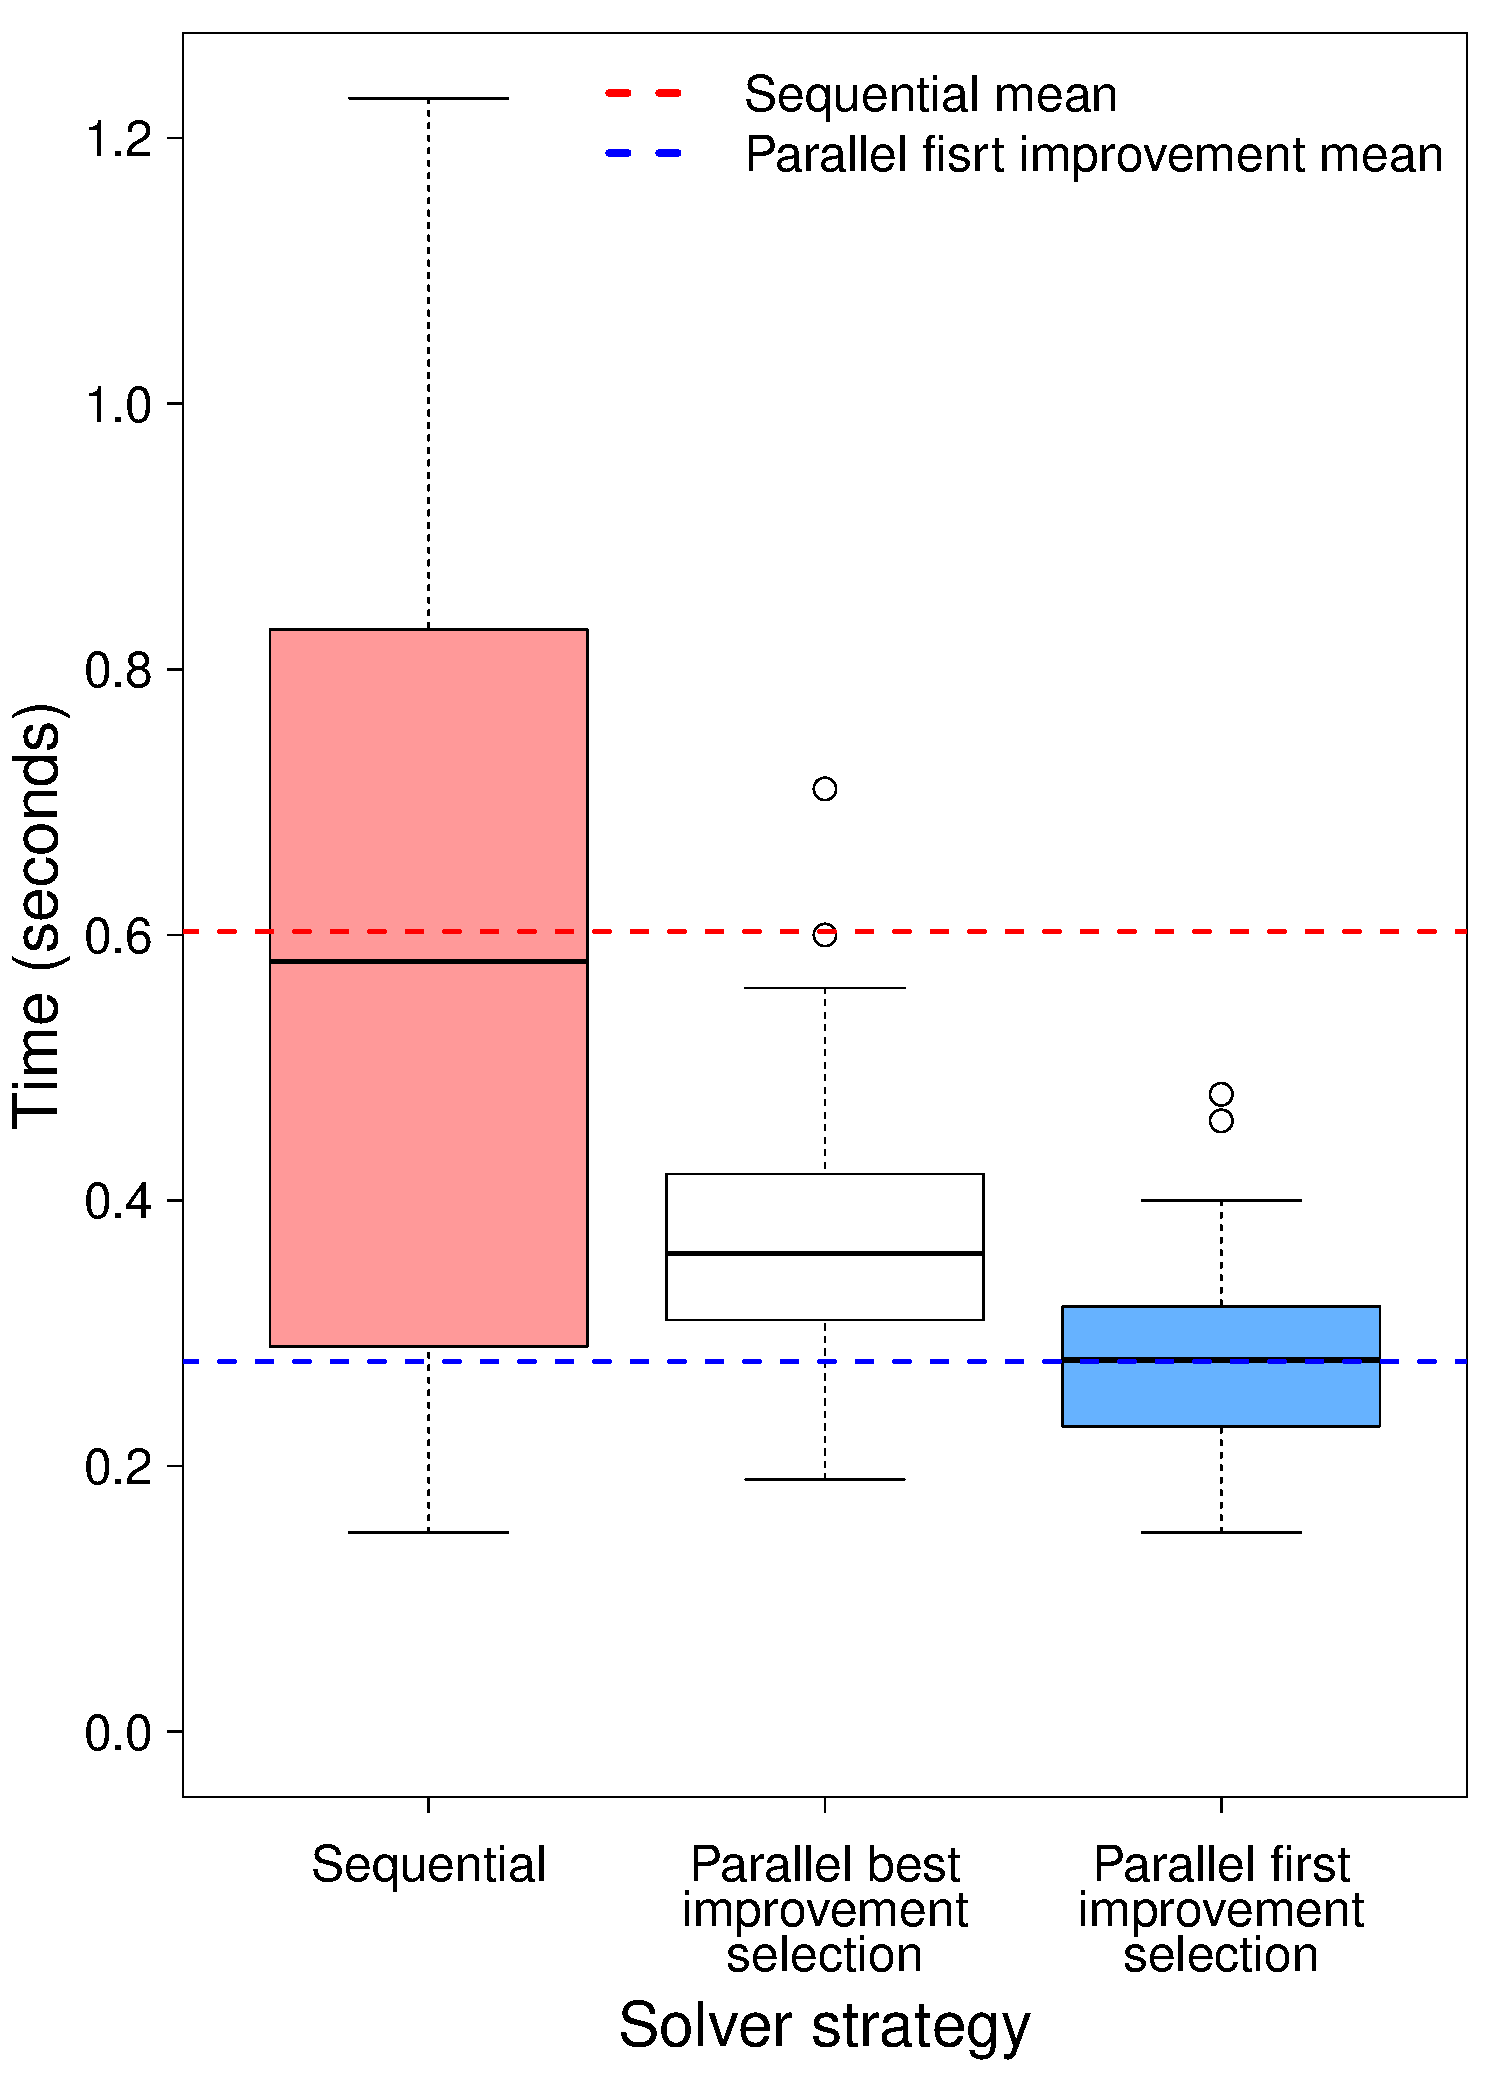
\includegraphics[width=0.75\textwidth]{g8_select_BP.pdf}
%\caption{Comparison between sequential and parallel (best improvement and first improvement selections) runs to solve \SGP{} 8-4-7 using \posl}
%\end{figure}

%\begin{figure}[!h]
%\centering
%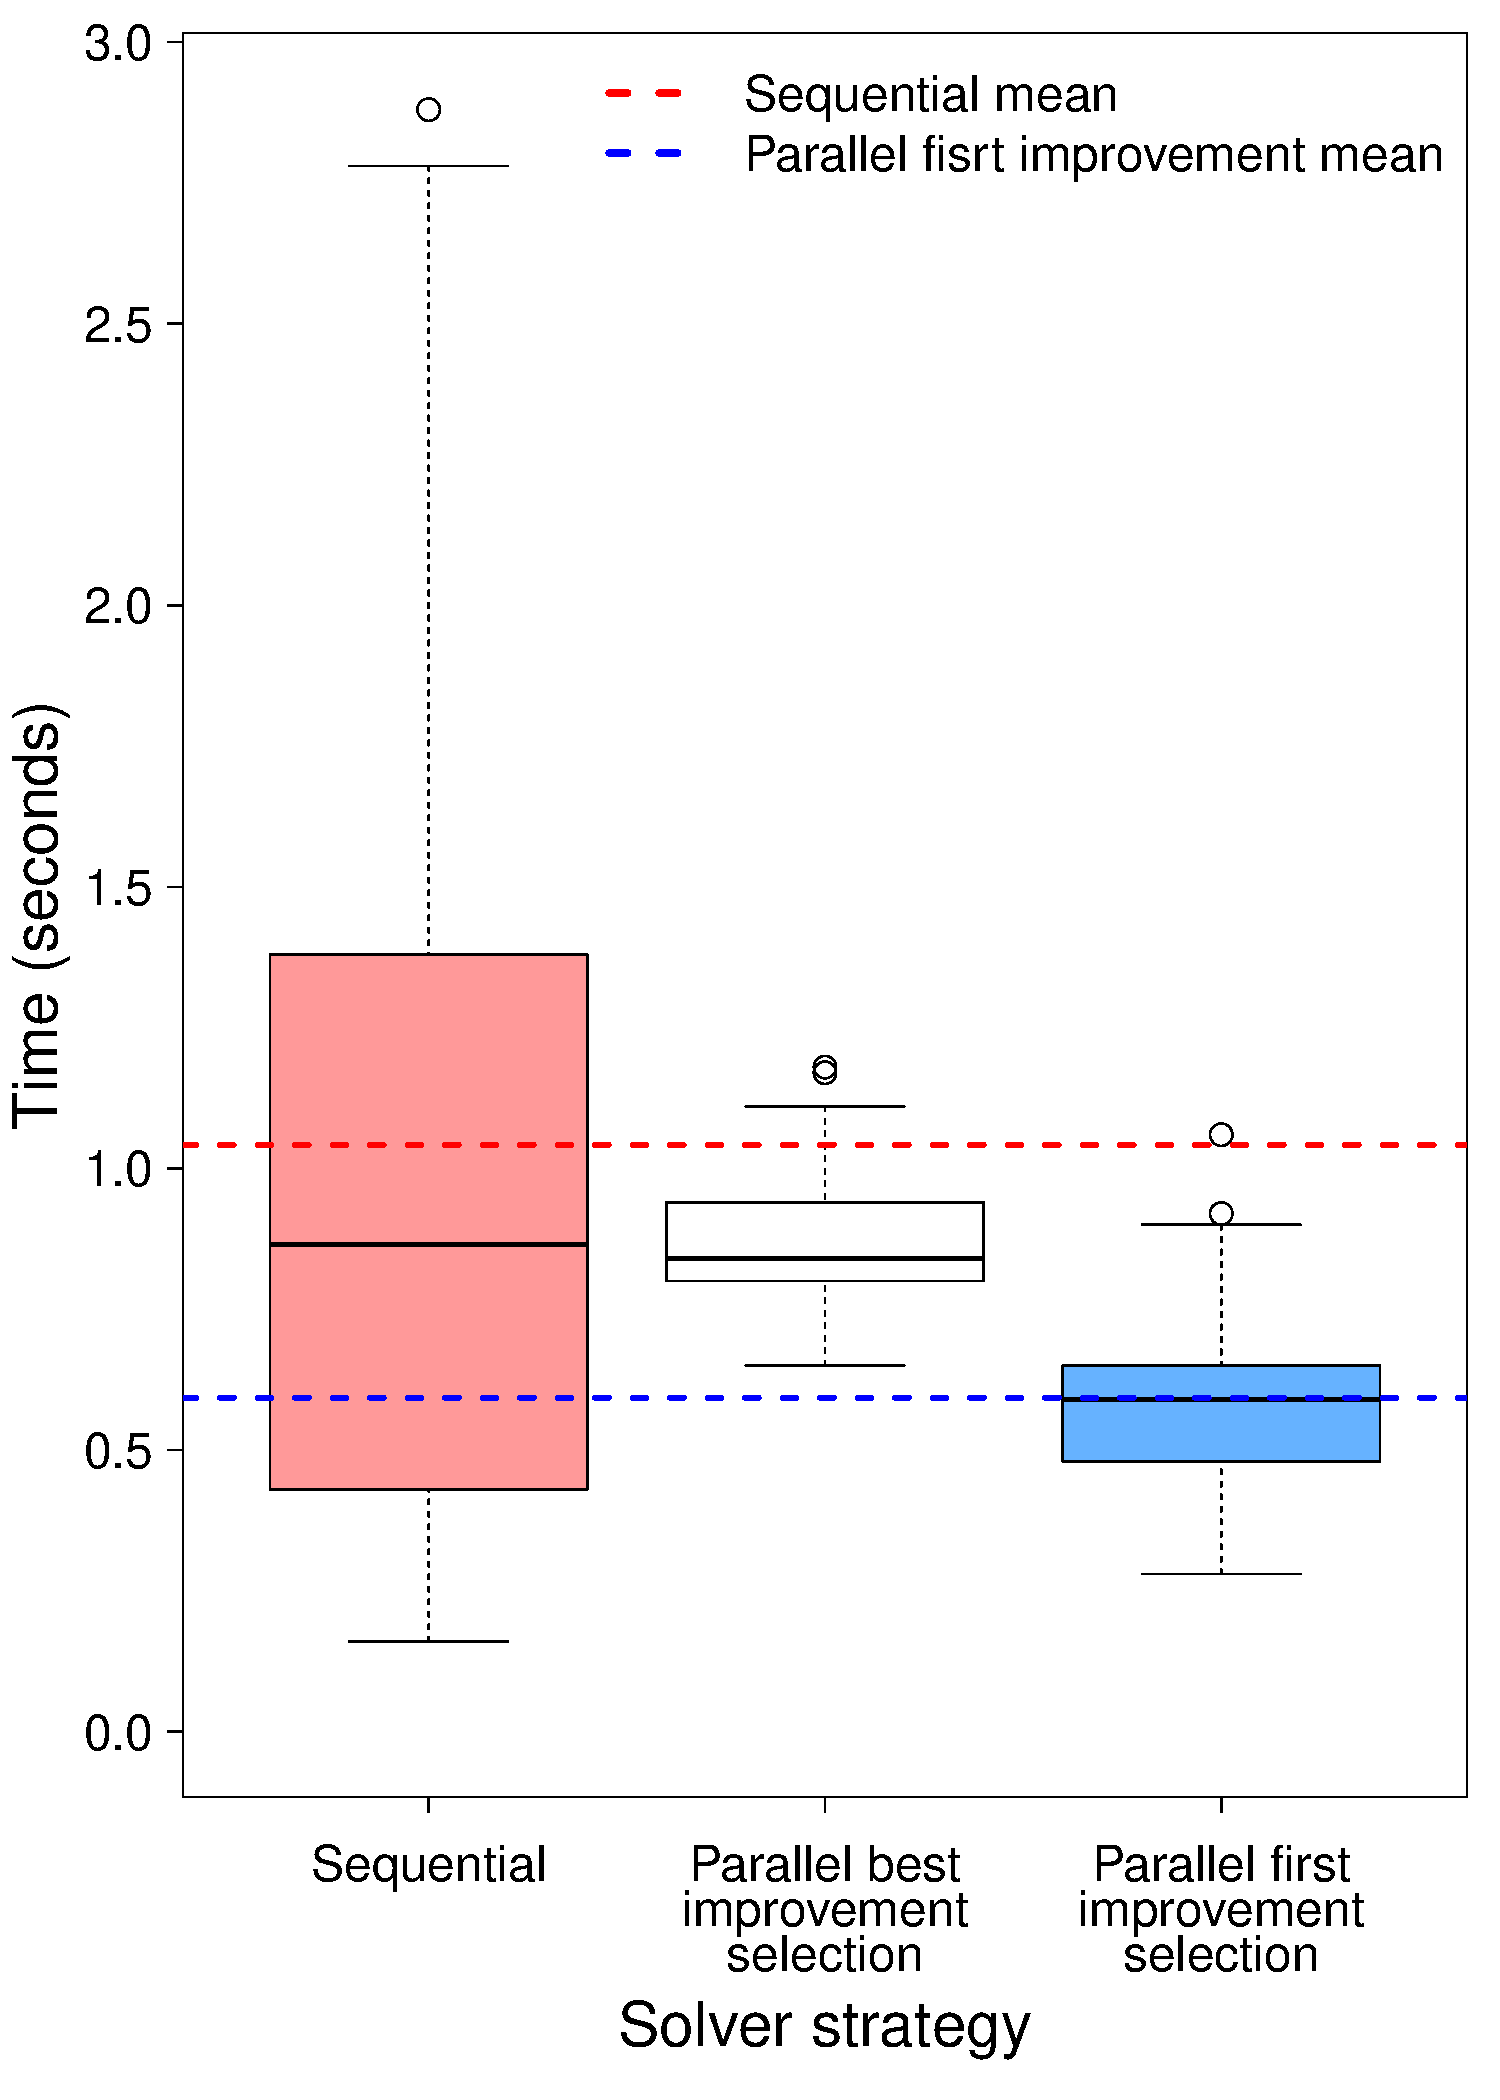
\includegraphics[width=0.75\textwidth]{g9_select_BP.pdf}
%\caption{Comparison between sequential and parallel (best improvement and first improvement selections) runs to solve \SGP{} 9-4-8 using \posl}
%\end{figure}

\section{Winner solver type representation}

Figures~\ref{barplot:5}, \ref{barplot:8} and \ref{barplot:9}, represent the percentage of winner solvers for each communication strategy according to four different types:

\poslcaptiondesciption{
\begin{tabular}[t]{rl}
\receiver{Receiver}: & Receiver solver wining thanks to the received information \\
\sender{Sender}: & Sender solver \\
\nonreceiver{Passive receiver}: & Receiver solver wining without using the received information \\
\nocomm{Non communicating}: & Non communicating solver \\
\end{tabular}
}

In these bar graphs it is evident to see that the communication has played an important role in the solution process. The number of receiver solvers which have won the search process is high, as expected, performing dynamic exchange strategies with communication \oneTn. However, due to the huge traffic of information, the communication overhead makes the resulting runtimes not competitive. 

The other interesting detail showed in these graphs is that this number of winner receiver solvers remains high on winner \commstrs{} (\texttt{100\%CC1-1} and \texttt{50\%CC1-1}), achieving an important trade-off between information traffic and search speed. 

%-------- SOLVER TYPE
\begin{figure}[!h]
\centering
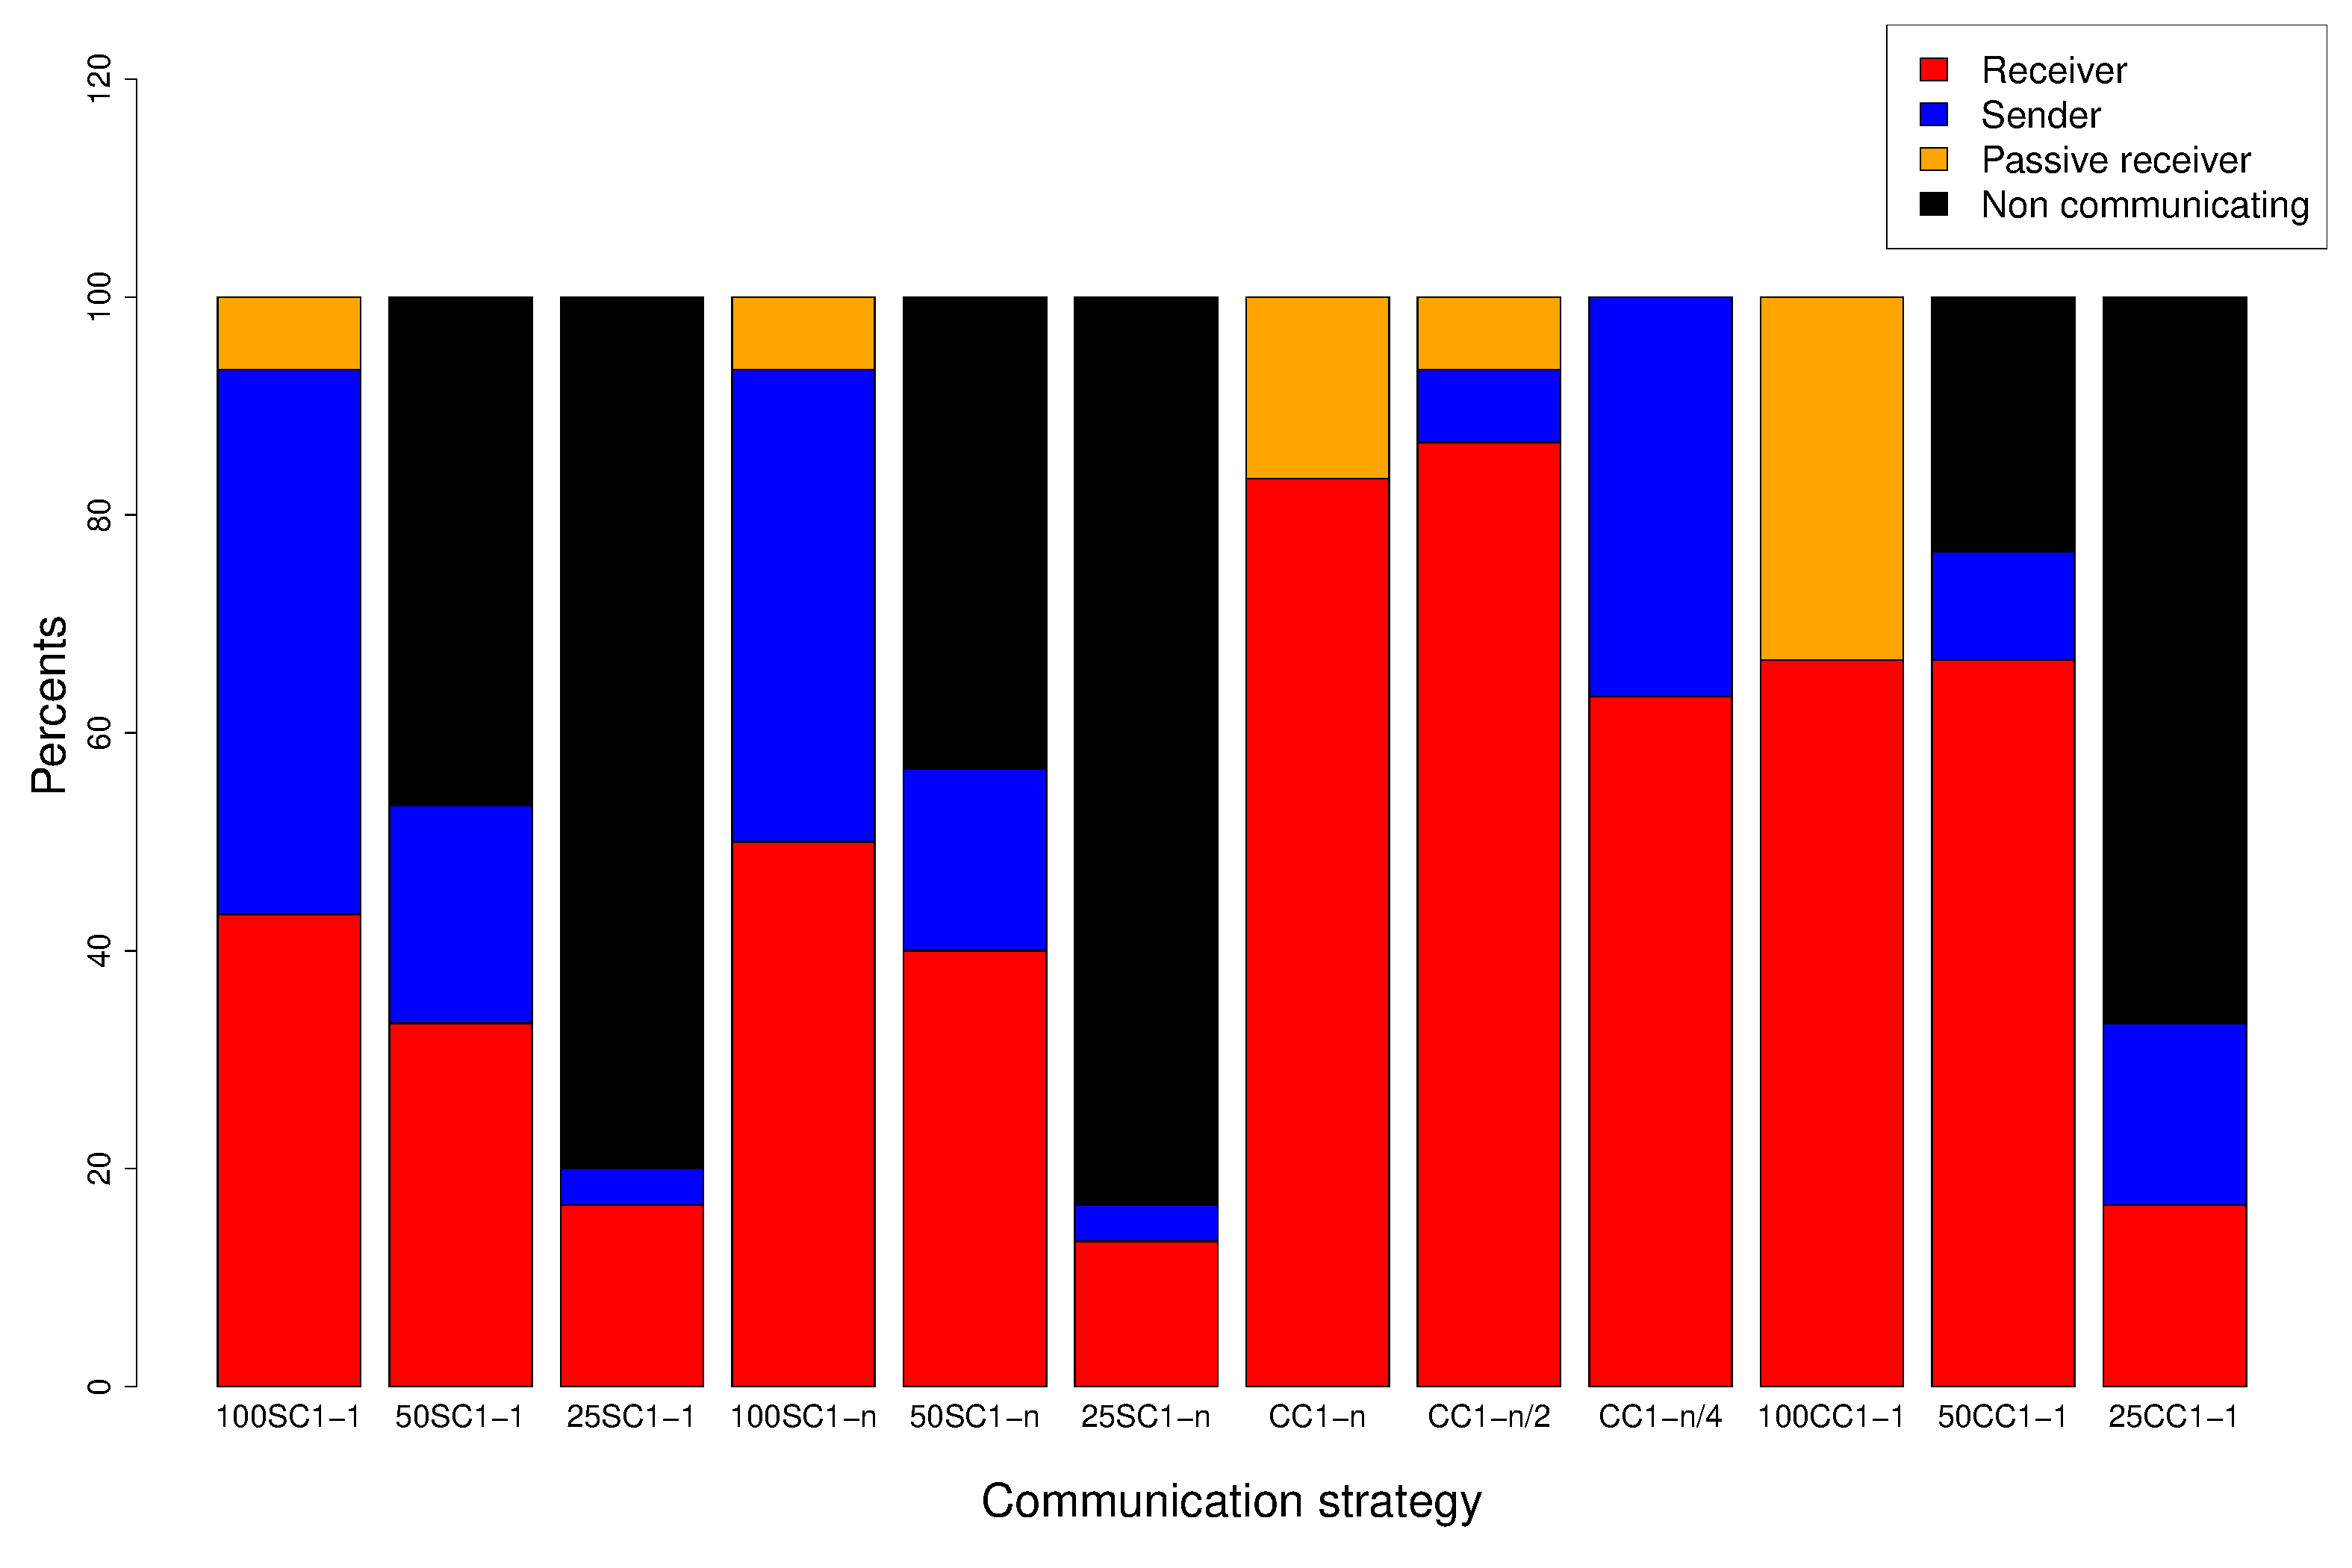
\includegraphics[width=0.8\textwidth]{g5_per_BP.pdf}
\caption{Solver proportion for each communication strategy to solve \SGP{} 5-3-7 using \posl}\label{barplot:5}
\end{figure}

\begin{figure}[!h]
\centering
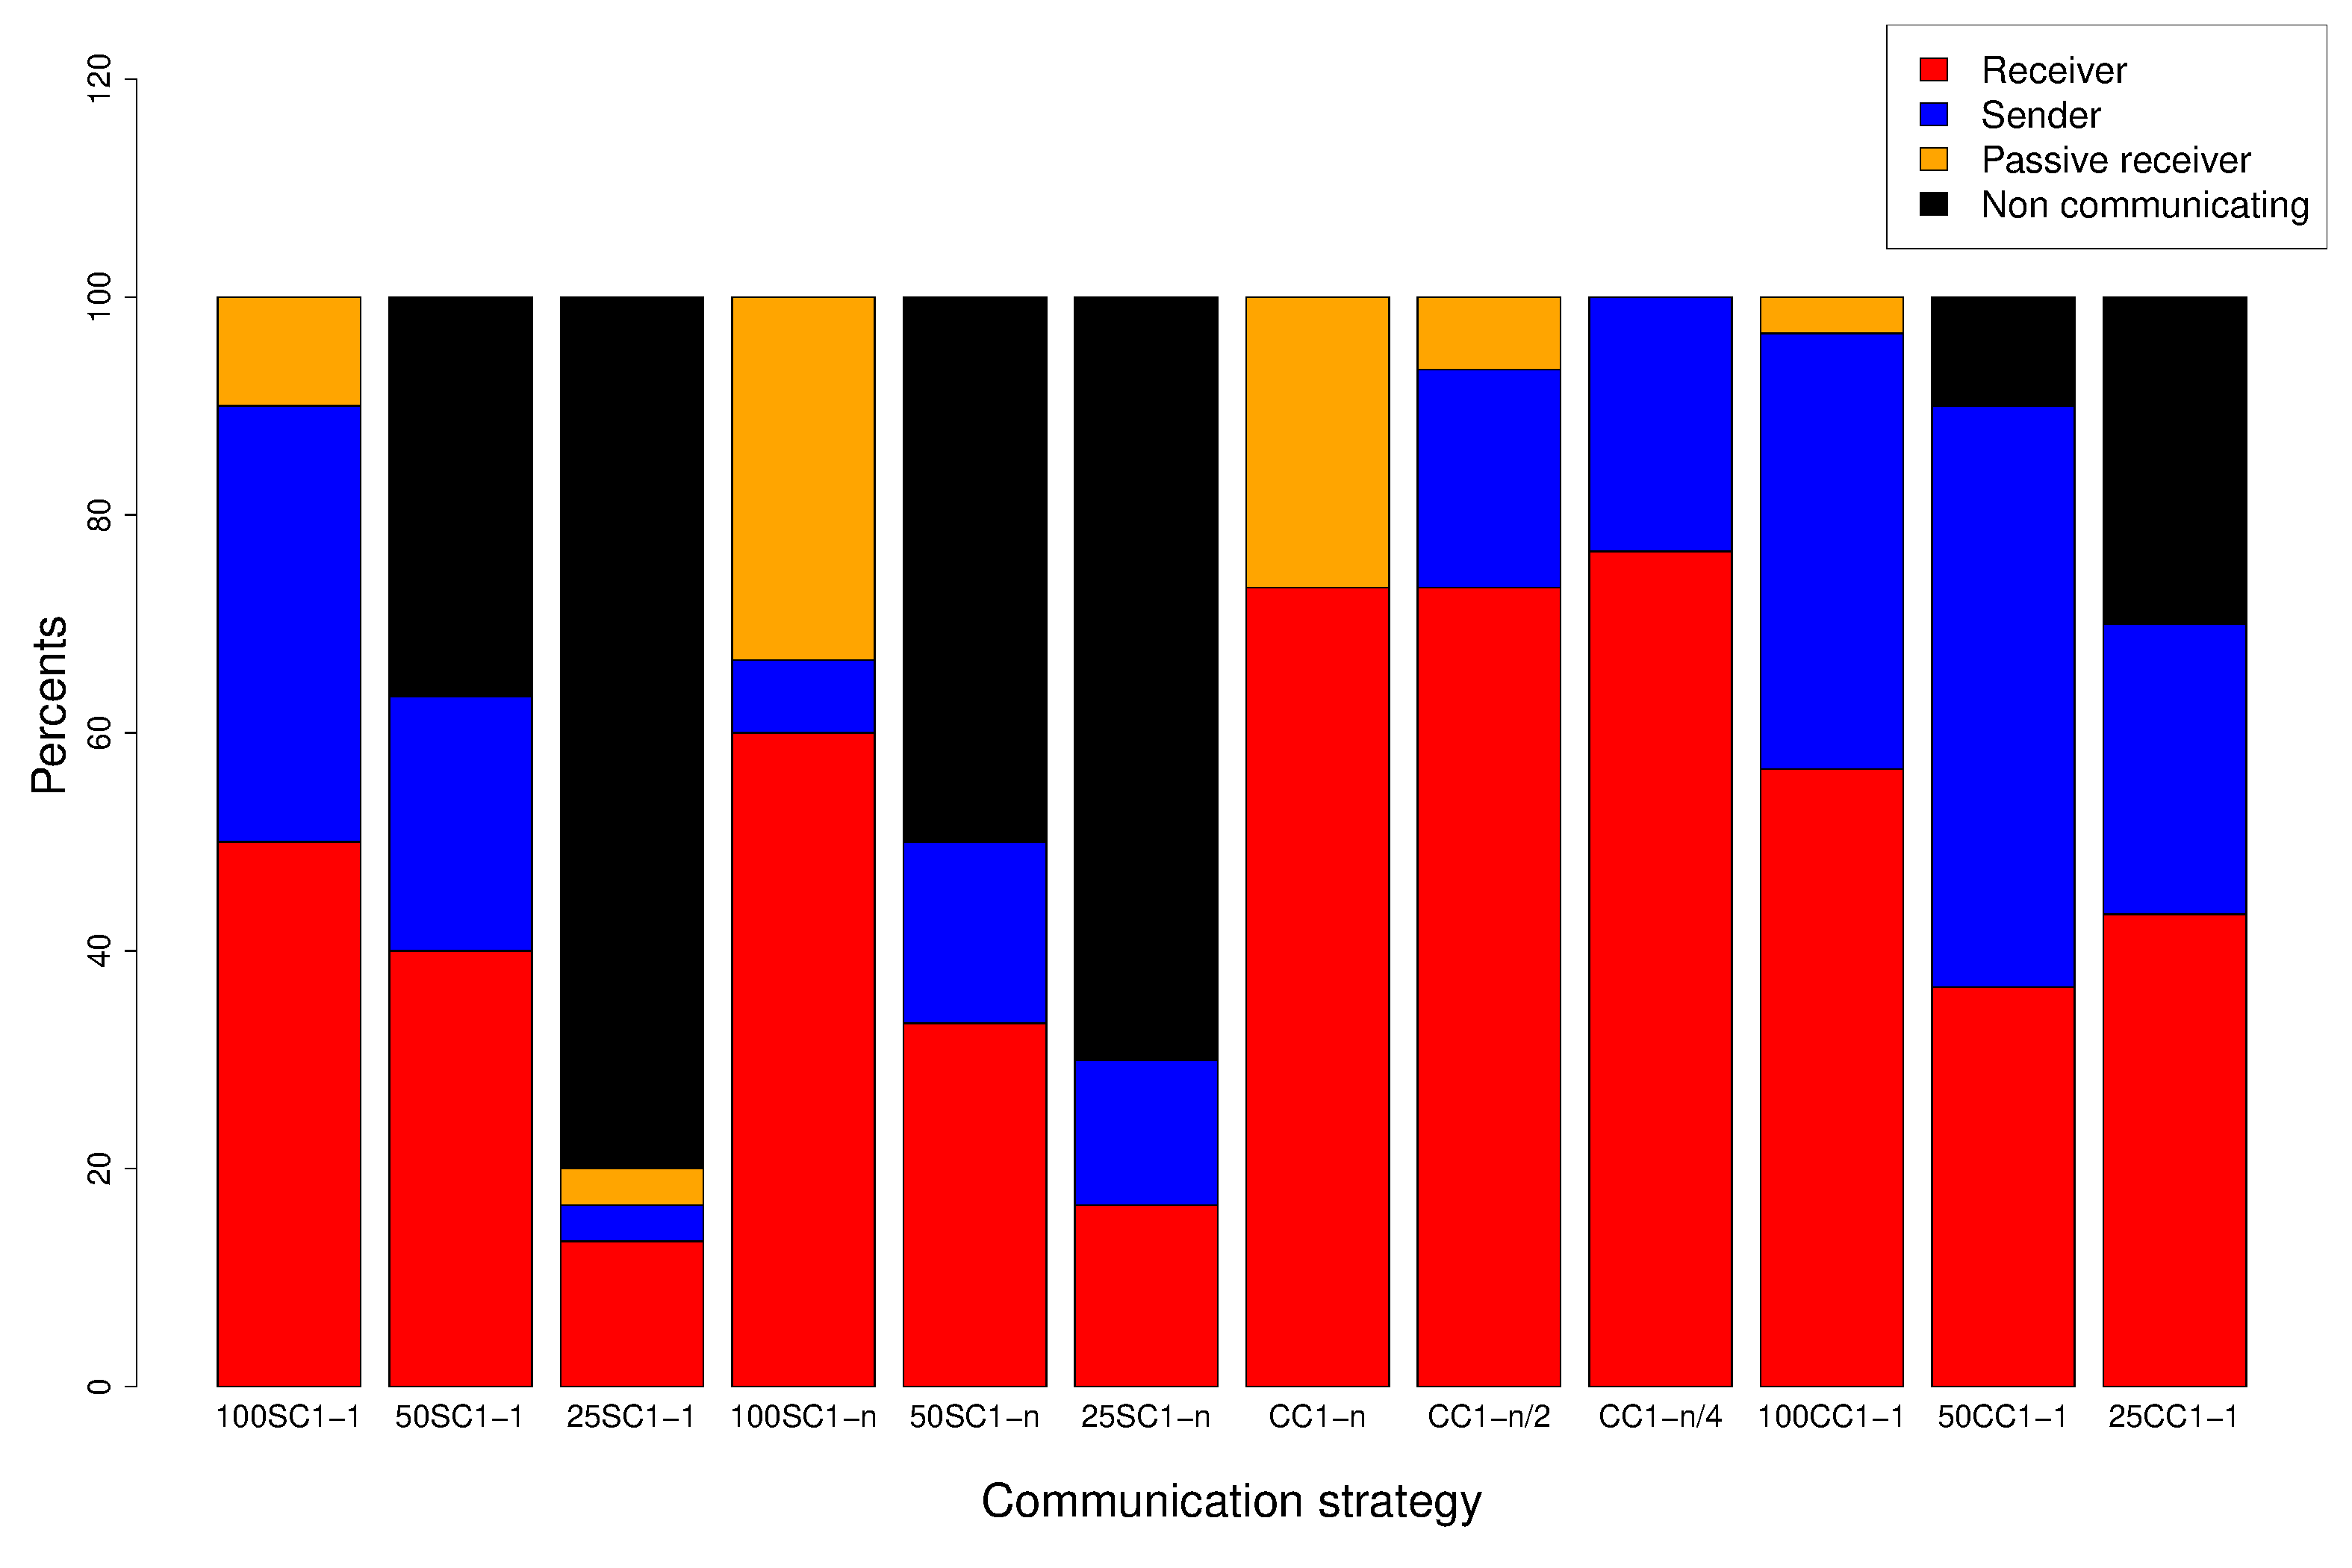
\includegraphics[width=0.8\textwidth]{g8_per_BP.pdf}
\caption{Solver proportion for each communication strategy to solve \SGP{} 8-4-7 using \posl}\label{barplot:8}
\end{figure}

\begin{figure}[!h]
\centering
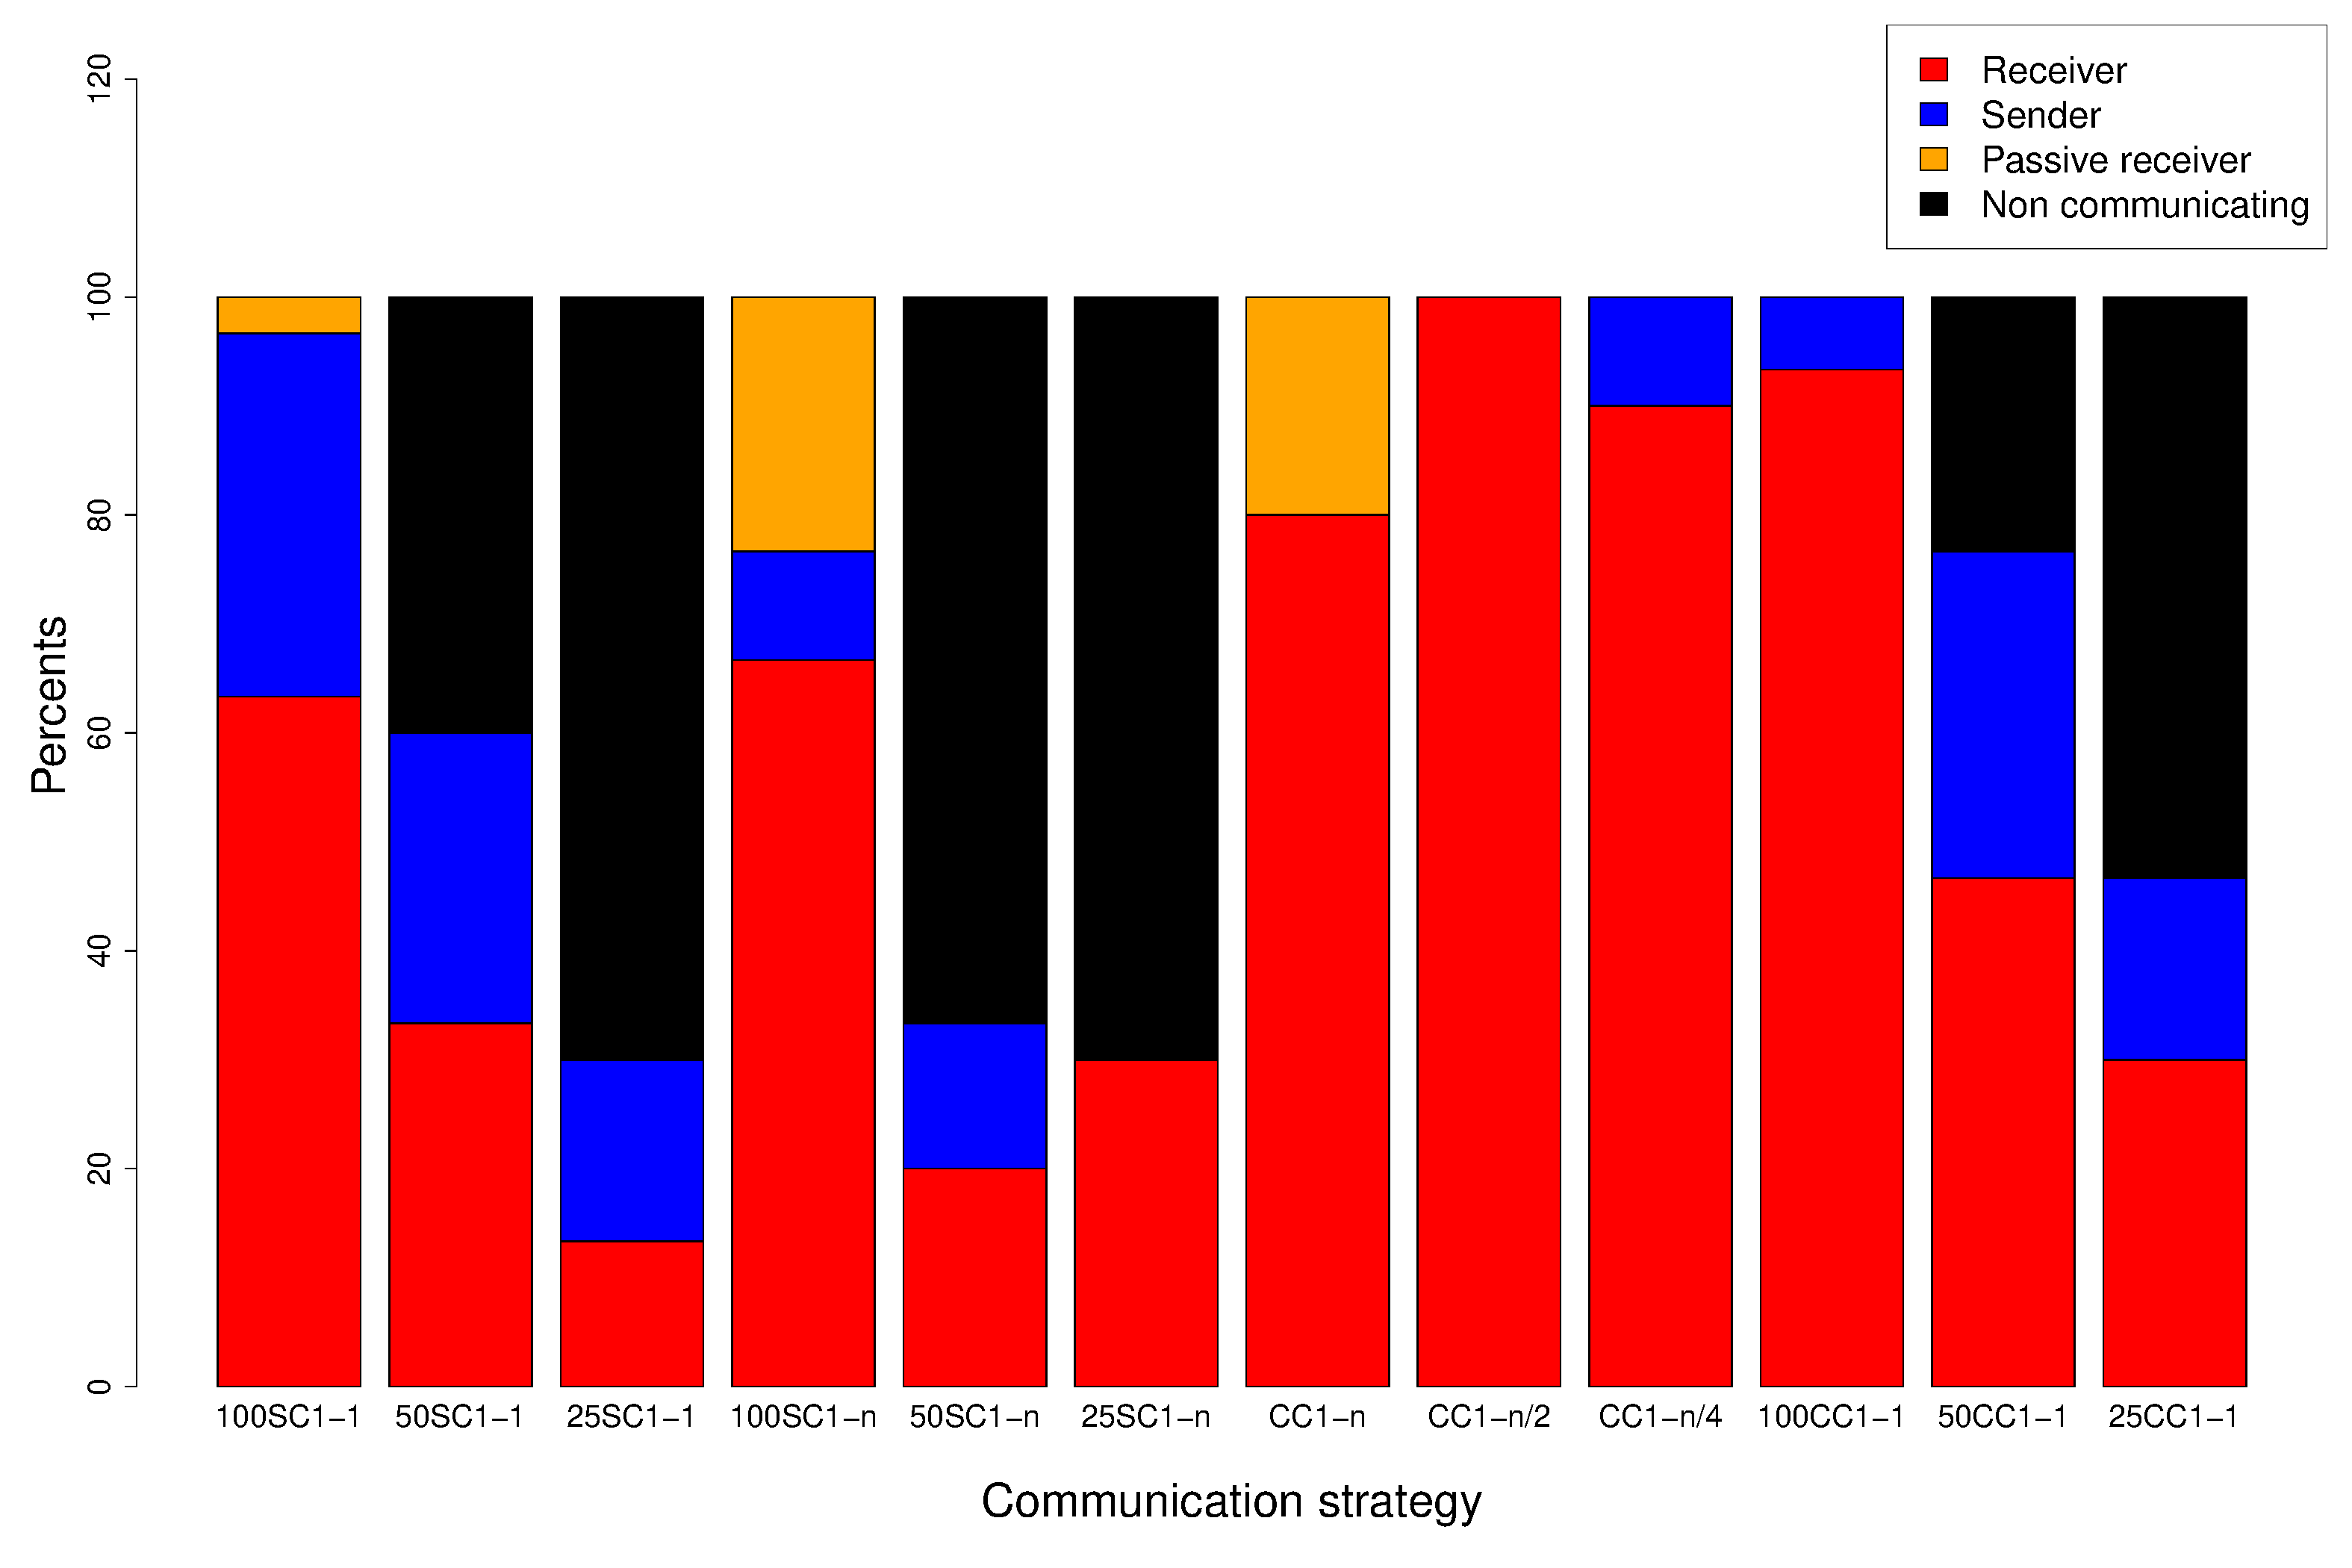
\includegraphics[width=0.8\textwidth]{g9_per_BP.pdf}
\caption{Solver proportion for each communication strategy to solve \SGP{} 9-4-8 using \posl}\label{barplot:9}
\end{figure}